\documentclass[oneside,a4paper,11pt]{report}
%\usepackage[T1]{slovak}
\usepackage[utf8]{inputenc}
\usepackage{latexsym}
\usepackage{graphicx}
\usepackage{amsmath}
\usepackage{amssymb}
\usepackage{caption}
\usepackage{fancyhdr}
%\usepackage{picins}
\usepackage{times}
\usepackage{mathptmx}
\usepackage{url}
\usepackage{booktabs}
\usepackage{appendix}
\usepackage{rotating}
\usepackage{hyperref}
\usepackage{verbatim}

\renewcommand{\chaptermark}[1]{\markboth{\thechapter.\ #1}{}}

\usepackage[Sonny]{fncychap}
\makeatletter
 \ChNameVar{\small}
 \ChNumVar{\LARGE}
 \ChTitleVar{\LARGE\centering}
 \ChRuleWidth{0.05pt}
 \ChNameUpperCase

\pagestyle{fancy}
\fancyhf{}
\fancyhead{}
\fancyhead[L]{\footnotesize \leftmark}
\fancyhead[R]{\footnotesize PAGE \thepage\ of XX }

\usepackage{hyperref}
\newcommand\araa{ARA\&A}
\newcommand\aap{A\&A}
\newcommand\apj{ApJ}
\newcommand\apjs{ApJS}
\newcommand\mnras{MNRAS}
\newcommand{\pasp}{Publications of the Astronomical Society of the Pacific}
\newcommand\ssr{Space Science Reviews}
\usepackage{natbib}
% The astroads bibtex style formats the references according
% to the well-estabilished syntax in use in astronomy and
% creates a link if URLs are specified for a given record.

\bibliographystyle{astroads}


%\title{Štúdium premenných hviezd vo vysokoenergetickej části spektra}
\title{On stars in high energy }

\author{Matúš Kocka}



\begin{document}
\thispagestyle{empty}
\begin{figure}
\begin{center}
\includegraphics[width=8cm]{plot/logo}
\end{center}
\end{figure}
\begin{center}
%\Large \textsc{MASARYKOVA UNIVERZITA} \\
%Přírodovědecká Fakulta

\vspace{2cm}
\Large 

\Huge On Stars in High Energies \\
\vspace{1cm}
\Large Matúš Kocka \\
\Large January 2012 \\
\vspace{2cm}
\LARGE Department of Theoretical Physics and Astrophysics \\
Masaryk University
\end{center}
\pagebreak



%\begin{figure}
%\begin{center}
%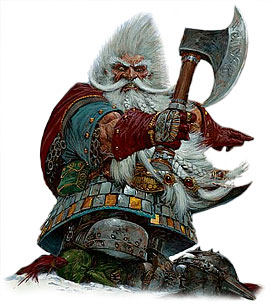
\includegraphics[width=6cm]{the-white-dwarf}
%\end{center}
%\end{figure}

\newpage
\textit{"Per aspera ad astra..."}

\pagebreak
\tableofcontents

\addcontentsline{toc}{chapter}{\protect\numberline{}Introduction}
\chapter{Introduction to the stars in high energy }

Let your imagination soar. 
Whe sitting on the old rocker looking at the sky with couple of good old whiskey you can easily 
start thinking about the universe. 
%You are looking at a heck of a different kinds of cosmic 
%objects, but suddenly you see almost only the stars. Almost all the shiny dots on the sky are 
%stars and these stars are only the closest ones. Yes, you can see few other 
%galaxies by naked eye\footnote{M31 and M33 in extremely good conditions on northern hemisphere
%and Magellanic clouds on southern one}, but none of the exotic cosmic objects you are imaging about. 
There are myliards of different kinds of cosmic objects, but what you see in the night sky are predominantly stars.
Indeed, almost all the shiny dots in the sky are stars, most of then being exceptionally bright and close - just a tiny
speck of the galaxy's total population. You may be able to spot a handful of other galaxies that are bright enough to 
be seen by the naked eye, however, all the exotic objects that we are imagination remain elusive.  
They are too faint to be observed easily, because they are not only far, far away, but they also usually shine 
on different wavelengths, not visible by the human eye.

Think about the distances in the universe. One of the most accurate explanations is the one from: \cite{hitch:1}  
\textit{"Space," it says, "is big. Really big. You just won't believe how vastly, 
hugely, mindbogglingly big it is. I mean, you may think it's a long way down the road to the 
chemist's, but that's just peanuts to space..."} 

Consider this, sometimes you want to study processes in these extreme, very faint objects, 
but they are too faint and too far out in the universe. You are looking for a “laboratory” with similar
 processes, but located much closer to the observer. The X-ray binary stars can be comsidered s this kind of 
laboratories.  

There are, of course, many interesting phenomena which could be studied in X-ray binaries or in non-binary X-ray stars. 
Several of them are mentioned in the motivation section. 

I am mentioning about several various space objects in this work, but the main effort is made to 
study the post-shock region in the Intermediate Polars (IPs).   


\section{Motivation}
We can easily find many reasons why to study stars in the high energy bands.  
We can consider the direct and the most common scientific applications like observations of 
the supernovae, black holes and neutron stars in X-ray binaries. But for the education purposes 
I prefer several other, very nice examples closer to the topic of this work.  

\begin{itemize}
 \item \textbf{Relativistic jet phenomena}: like it was proposed by \citet{mirabel:1} that the universal 
mechanism should be at work in all the relativistic jet sources in the universe. Better understanding 
of sources including: microblazars, AGNs and gamma-ray burst will help to gain a more comprehensive 
understanding of these phenomena. Microblazars can play a role of “space laboratories”, where interesting
 processes last on different timescales as is the case with AGNs or GRBs.   

\begin{figure}[!hbt]
\centering
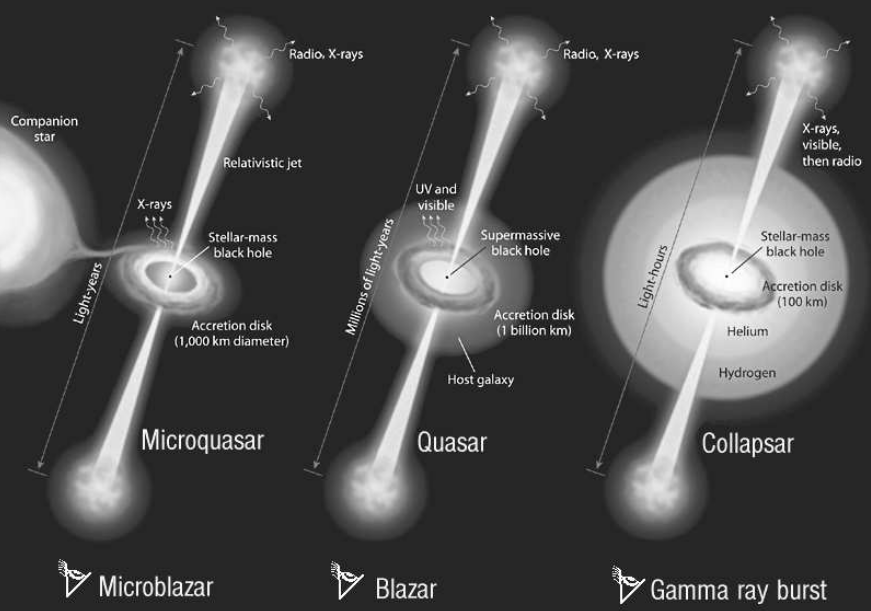
\includegraphics[totalheight=8.5cm]{microblazars}
\caption{NOT in scale diagram, showing current ideas of micro-quasars, AGNs and gamma-ray
bursts as space objects driven by the same, universal mechanism  \citet{mirabel:1}. }
\label{microblazar} 
\end{figure}

 \item \textbf{Galactic ridge X-ray emission (GRXE)}: various physical processes contribute to 
brightness of GRXE in different bands, but several studies in 3-20 keV provide evidence that the diffuse 
X-ray radiation originates from a huge number of stellar X-ray sources, mostly coronally active stars
 and white dwarf X-ray binaries. In particular for the energies over 20 keV to 200 keV, the spectrum is
very similar to the spectrum of magnetic white dwarf binaries – e.g. Intermediate polars (IP) and polars (P).  
\citet{2007A&A...463..957K}
 
 \item \textbf{White dwarfs' masses in Intermediate Polars (IP)}: as was proposed in \citet{1981ApJ...250..723R}, 
the temperature of the post shock region (PSR) depends on WD mass. Therefor the X-ray spectrum can be 
used for WD mass determination \citet{2005A&A...435..191S}. The WD mass estimations in cataclysmic stars 
is in general complicated. Usually, the curve of radiation velocities can be used, but it is quite hard to constuct. 
Therefore the X-ray spectrum method is very atractive for several reasons. This work is dedicated to this topic.  

\end{itemize}

\section{Aim of this work}
To cover the whole topic: ``stars in high energies'' is far behind a capacity of a master thesis and because of that I have decided 
to concetrate on cataclysmic variable stars (CVs), especialy on intermediate polars (IPs). 

As it will be mentioned in the next sections closely, IPs are magnetized CVs where the compact, primary star 
is a white dwarf with $B\sim 10^6 -10^7$ Gauss. The mass accretion is taking place from, mainly a low-mass, non-degenerate star through its Roche lobe.  
The accretion disk is in some distance from the WD surface destroyed by a strong magnetic field and 
the accretion continues through, the so called, accretion curtain across the magnetic force-field.

The falling material in some point creates a stationary shock near the WD surface where the kinetic energy is converted 
through thermal bremsstrahlung to radiation. The temperature of the created plasma is typically more than 
10 keV with a low density. The optically thin hard X-ray\footnote{In this case, hard X-rays means 10 - 120 keV region.} emission is taking place and heated gas creates the 
post-shock region (PSR) with temperature gradient. The hot gas then descends and cools by the X-ray 
emission while it hits the WD surface.      

Because of the relatively high temperature of PSR are IPs very well observed in hard X-rays band. 
IPs comprise only a small fraction $\sim 15\%$ of all CVs, but they dominate in hard X-ray band over 10keV, at most 
$\sim 80\%$ of detected CVs are IPs \citet{2009MNRAS.392..630L}. 

The temperature of the PSR depends in first order only on the WD mass, which is the most fundamental parameter of WDs.
This means, that if we are able to find temperature from fiting the thermal bremsstrahlung model to a spectrum of IP, 
we are also able to establish the WD's mass. 

The accreting WDs are very important for cosmology, because some of such objects probably cause Type Ia supernovae, 
when the WD mass reaches Chandrasekhar limit. 

As is showed on fig.(\ref{nylup1}), IPs as NY Lup are well observed by INTEGRAL/IBIS detector which makes them 
interesting space laboratories to investigate the basic parameters of WDs. In same casesm, can by also accretion stream studied
if it is strong enough. 
    


\begin{figure}[!hbt]
\centering
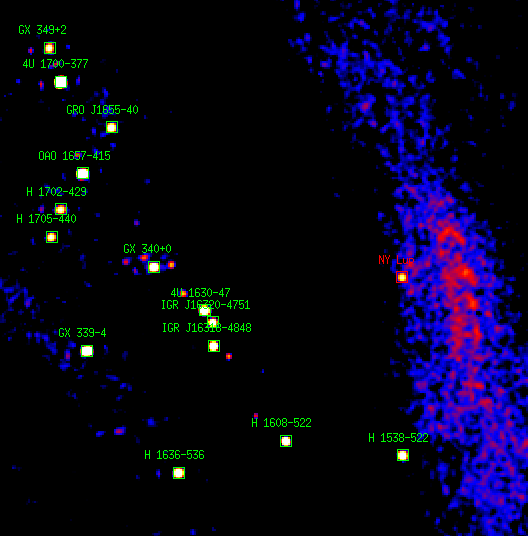
\includegraphics[totalheight=12cm]{plot/ds9_3}
\caption{1.2 Msec exposure of NY Lup region in 17-80 keV. The NY Lup is marked by red square. There are many others X-ray sources,
mostly HMXBs or LMXBs.}
\label{nylup1} 
\end{figure}



\section{Observations}
Cataclysmic Variable stars (CVs) have been, in fact, observed as early as the ancient times. In the historical 
records of  many civilizations we can find references for various astronomical events. Most of them are about objects
that exhibits periodic variations of a some type, most notably: planets, Moon and Sun. However several of them are about comets and new stars.  
These new stars are in many cases novae and supernovae. In China, the records date back to 1500 BC. 

Many records are saved from the medieval time, for example positions of Nova Vulpecula 1670 and 
Nova Cygni 1600 (now knows as P Cygni) in Hevelius maps. 

With the advent of astronomical photography in the late 19th century started the era of continuous observations
and with the development of first photo-multipliers in the mid-1940s CVs begun to be attractive 
targets because of their big variability in the different time scales. 

The AAVSO has light curve of SS Cyg from 1896 up to date. 

\subsection{Optical and IR observations}
The very first visual observation was followed by the photographic photometry and then spectroscopy, 
followed by the photo-multiplier photometry since mid-1940s. The binary nature of all CVs was confirmed. 
The flickering was discovered and was assumed that it is somehow connected to stars' duplicity Walker (1957),
\citet{warner:1}.

Statistical studies by Luyten and Hughes in mid-1960th showed, that novae remnants have $M_V \approx 4$ and 
dwarf novae at quisence have $M_V \approx 7.5$. They conclude that the hot primary star in CVs must be WD or 
 hot subdwarf \citet{warner:1}.   

The most important contribution of optical astronomy to this work is the discovery of large and 
variable circular polarization in several CVs. This helped to identify magnetic CVs, 
which were later divided to two categories, polars and intermediate polars.

There are more important discoveries in optical and IR bands in CVs subject. In the case of interest the 
 \citet{warner:1} is te recommended book. 
   
   
\subsection{X-ray observations}
The very first CV detected in X-rays was EX Hya observed by Uhuru X-ray space mission. 
Uhuru worked in 2.0 – 6.0 keV and in spite of its poor sensitivity the well-known 4U catalogue
 was created \citet{1978ApJS...38..357F} from its observations.

The NASA`s HEAO\footnote{High Energy Astronomy Observatory, The HEAO 2 was also known as 
The Einstein Observatory} program followed with three space missions. As the X-ray detectors 
technology evolved, the number of detected CVs growed linearly. \mbox{EXOSAT} provided long and 
uninterrupted data for many CVs during its operation from May 1983 until April 1986. 
Similar results were obtained from Soviet mission \mbox{Kvant 1} and Japan's Ginga.
The high hopes were invested into ROSAT which provided the all-sky survey in the
 0.1 – 2.0 keV but the expected huge number of new CVs was not discovered. 

The situation slightly changes with RXTE\footnote{Rossi X-ray Timing Explorer} which after several 
years on orbit provided good data for several articles about WD masses \citet{2005A&A...435..191S}. 
The data from RXTE are used in the new articles even $\sim15$ years after its launch \citet{2011A&A...526A..77B}.
 
Several others missions were launched in the last ten years period. Few of them carried several 
detectors where one was sensitive in X-rays, like SUZAKU/XIS and Swift/XRT. But for the X-ray 
astronomy the year of 1999 was the most important so far. The two major big observatories 
were launched on the Earth's orbit. The Chandra X-ray Observatory flew onboard STS-93 space shuttle 
Columbia on July and the XMM-Newton was launched onboard ESA's Ariane 5 rocket.

   That was the beginning of the X-ray astronomy's golden era. During the last decade the combination of 
Chandra and XMM provided enormous data archives which will be useful for astronomers in another 
decades. 

Sadly, there is no big X-ray observatory planned for the next decade. One of the bigger space 
mission will be Japan's ASTRO-H with several X-ray and gamma ray detectors on-board to cover broad 
high energy bands. The future of big ESA \& NASA space mission Athena (formerly: Constellation-X, 
XEUS, IXO)  is questionable because of budget cuts in both space agencies. 

Fortunately, there are several data archives with open acces for anybody 
interested. This is a big challenge mainly for young astronomers, who are 
not directly involved in any big space mission program but want to do science. In this case, 
they don't need any special hardware, even modern laptops are powerful enough.     



    
\subsection{Gamma ray observations}
In last millennium several space mission observed few CVs in bands from tens of keV to TeV.\footnote{The most 
studied CV from this era is AE Aqr (Meintjes 1990; Bowden et al. 1991)}
The biggest breakthrough came with ESA's INTEGRAL space mission which was able to observed many CVs with its
exceptional sensitivity and large field of view. Mostly intermediate polars. Only $\sim 2\%$ 
of all CVs are actually magnetic ones, but these ones are only visible in gamma rays.
INTEGRAL/IBIS was been used to determine white dwarf masses by \citet{2009MNRAS.392..630L}.

Two others space missions have on-board detectors similar to INTEGRAL/IBIS with their sensitivity 
and coverage: the NASA's Swift/BAT and Japan's Suzaku/XRT. Both are widely used to study white dwarf 
masses in IPs \citet{2009A&A...496..121B}, \citet{2010A&A...520A..25Y}.    



\chapter{White Dwarfs}
White dwarfs born when normall mass stars die. WDs are degenerated, late type stars with typical mass $\sim 1 \mathrm{M_{\odot}}$. Their typical radius is about
 5000 km and mean density around $10^6 \mathrm{g\:cm^{-3}}$ (\citet{2004bhwd.book.....S}). They no longer burn nuclear fuel and
if they don't have any other mather influx e.g. by accretion from close star, they slowly cools as they radiate
away residual thermal enegy.

WDs support themselves against gravity by the pressure of electron degenerate gas and theyr interior is in the local thermal 
equilibrium, except the thin atmosphere.  

\section{First look of white dwarfs interior}
WDs are a class of the less compact objects among the possible endpoints of the stellar evolution. 
The mass of the star is the main factor determining whether the star ends up as a WD, neutron star or a black hole.
The medium mass stars with masses $\mathrm{M} \lesssim  4\mathrm{M_{\odot}}$\footnote{Also $\mathrm{M} \lesssim  8\mathrm{M_{\odot}}$ can be find in 
some literature, \citet{padm_vII}.} in some point of late state of their evolution gently spreads mass
 forming planetary nebulae. The rest of the star become the white dwarf.  

\begin{table}[hbt!]
\caption{Basic statisticks of the compact objects \citet{2004bhwd.book.....S}}
\centering
\begin{tabular}{lllll}
\hline
\hline
Object & Mass$^a$ & Radius$^b$ & Mean Density & Surface Potential  \\
       & $[\mathrm{M]}$ & $[\mathrm{R]}$ & $[\mathrm{r\:cm^{-3}]}$& $[GM/Rc^2]$                    \\
\hline
Sun         & $\mathrm{M_{\odot}}$            & $\mathrm{R_{\odot}}$             &1                  &$10^{-6}$ \\
White Dwarf & $\lesssim \mathrm{M_{\odot}}$   & $\sim 10^{-2}\mathrm{R_{\odot}}$ & $\lesssim 10^7$   &$\sim 10^{-4}$ \\
Neutron Star& $\sim1-3\mathrm{M_{\odot}}$     & $\sim 10^{-5}\mathrm{R_{\odot}}$ & $\lesssim 10^{15}$& $\sim 10^{-1}$\\
Black Hole  & Arbitrary              & $2GM/c^2$               & $\sim M/R^3$      & $\sim1$\\
\hline
\footnotesize
$^a \mathrm{M_{\odot}}=1.989 \times 10^{33} \mathrm{g}$ &&&& \\
\footnotesize
$^b \mathrm{R_{\odot}}=6.9599 \times 10^{10} \mathrm{cm}$ &&&& \\
\end{tabular}
\label{comobj1}
\end{table}

Let's use data from the table \ref{comobj1} and try to assume the pressure inside of WD. For very 
rough estimation, we can use equation of mechanic equilibrium to compare WD with the Sun:

\begin{equation}
 \mathrm{d}P = -G\frac{M \varrho  \mathrm{d}r}{r^2},\:m(r) = \int_{0}^{r}\rho 4 \pi r^2 \mathrm{d}r \:.
\end{equation}

The ratio between variables $\mathrm{P,\: M,\: \rho}$ and $\mathrm{r}$ in the Sun case and $\mathrm{P', \:M',\: \rho',\: r'}$ in the WD's 
case can be written as follows:

\begin{center}
 $M' = M ,$  \\
 $r' = 10^{-2}r,$ \\
 $\rho' = 10^6 \rho,$ \\
\end{center}

From easy calculation we get: 
\begin{equation}
 \mathrm{d}P' = -G\frac{M' \rho' dr'}{r'^2} = -G\frac{M \cdot 10^6 \rho \cdot 10^{-2} \mathrm{d}r}{r^2 (10^{-2})^2} = 10^{8} \mathrm{d}P
\end{equation}

From such results is eminent that there is something wrong with the WDs interior in comparation with central reion of the 
normal star. As the ionization is increasing by higher temperatures, the bigger pressure otherwise helps recombination. However 
very big pressure actually increase ionization up to totally ionized atoms. Atoms without their 
electrons shells are closer to each others which explains very high density.

For densities in range $10^5 \mathrm{g\:cm^{-3}} \lesssim \rho \lesssim 10^9 \mathrm{g\:cm^{-3}}$ the WD is made 
of ideal nondegenerate gas of ions and a degenerate gas of electrons. The system will be degenerate 
if $T>T_c$ where $T_c \approx 3 \times 10^9 K (\rho / \rho_c)^{2/3} $ 

If the electrons are relativistic or not can be found by comparing $m_e c$ with a fermi momentum
\begin{equation}
 p_F = (3\pi^2)^{1/3}\hbar n_e^{1/3} = (3\pi^2)^{1/3}\hbar (\rho/\mu_e)^{1/3}
\end{equation}
 where 
\begin{equation}
 \mu_e = (\rho / n_e m_p) = 2(1+X)^{-1}
\end{equation}
is the mass per electron. The fermi momentum will be equal to $m_e c$ at the critical density:
\begin{equation}
\rho_c \equiv \frac{8\pi}{3}m+p \mu_e \frac{m_ec^3}{h} \approx 10^6 \mathrm{\mu_e\:g\:cm^{-3}}
\end{equation}

If the density is higher than $\rho \gtrsim 10^9 \mathrm{g\:cm^{-3}} $, the electrons are combined with protons inside of nuclei and 
create different matter called neutron degenerated gas. This is how neutron stars are made.    
 
\section{Fermi energy}
Now we can imagine interior of WDs as an area full of atoms nuclei very close to each other 
with free electrons around them. But electrons are fermions, which means that they must 
behave according to Pauli exclusion principle and it allows only at most one fermion 
per each quantum state. 

If we imagine a normal, everyday gas at standard temperature and pressure, only one 
of every $10^7$ quantum states is occupied by gas particles, so Pauli exclusion 
principle limitation is very insignificant. When energy is removed from the gas and 
it's temperature falls down, an increasingly large fraction of  the particles been 
forced into the lower energy states.

For fermions gas only one particle can take the lowest energy state and others must 
take another, higher and higher states, thus only one particle per state is allowed. 
Even in limit $T\rightarrow0$ pressure is produced by motions of electrons on excited positions.       

At the zero temperature all of the lowest states and none of the higher states are 
occupied, this kind of fermion gas is called completely degenerated. 
The max energy of electron in completely degenerate gas at $T=0 \mathrm{K}$ is known as Fermi energy. 

For determining the limiting energy we can imagine 3D box where length of each of its sides will be \textit{L}.  
The wavelengths of electrons trapped in the box in each dimension will be
\begin{equation}
\lambda (xyz) = \frac{2L}{N{(xyz)}}
\end{equation}
where $N_{xyz}$ are integer quantum numbers for each dimension. The momentum can be written 
through de Broglie wavelength
\begin{equation}
p(xyz) = \frac{hN(xyz)}{2L}
\end{equation}
We can now write the total kinetic energy of the electron when $p^2 = p_x^2 + p_y^2 + p_z^2$ as follows
\begin{equation}
\label{ferm1}
 \varepsilon =  \frac{p^2}{2m} \Rightarrow \frac{h^2N^2}{8mL^2}
\end{equation}
Total number of electrons is same as total number of unique quantum numbers $N_x, N_y, N_z,$ multiply by 
factor two. The two factor comes from the fact that electrons are particles with spin, which can be $\pm 1/2$. 
This means that two electrons are allowed to have the same tree quantum numbers but different spin. 
The total number of electrons out to radius $N = \sqrt{N_x^2 + N_y^2 + N_z^2}$ will be
\begin{equation}
 N_e = 2\left ( \frac{1}{8} \right )\left ( \frac{4}{3} \pi N^3\right ) \Rightarrow N = \left ( \frac{3N_e}{\pi} \right )^{1/3} .
\end{equation}

By using Eq. \eqref{ferm1} and simplifying it, we will get the Fermi energy as follows
\begin{equation}
\varepsilon_F = \frac{\hbar^2}{2m}\left ( 3\pi^2n \right )^{2/3}
\end{equation}
where $m$ is the mas of the electron or any other fermion\footnote{Can by applies for any fermion, not only electrons} 
and $n\equiv N_e/L^3$ is the electron count per volume. 
The average energy per electron at $T = 0\mathrm{K}$ is $3/5\varepsilon_F$.    
  
\section{Degeneracy}
Matter inside of WD has very symmetric spherical distribution, we can calculate the mass interior to radius $r$ like\footnote{More elaborate and precises approach can by find 
\citet{2004bhwd.book.....S}, \cite{padm_vII}, \citet{kleczek}, \citet{comp_obj1}, \citet{1972ApJ...175..417N} and simpler explanation with
less math in \citet{2007ima..book.....C}}
\begin{equation}
 \frac{\mathrm{d}m(r)}{\mathrm{d}r} = 4 \pi r^2 \rho
\end{equation}
In normal case the WD is in steady state and gravitation force is balanced by the pressure at every point.  
For deriving the hydrostatic equilibrium equation we need to consider an infinitesimal element laying between 
$r$ and $r+\mathrm{d}r$ with an area $\mathrm{d}A$. The element is lying perpendicular to the radial direction, should looks like fig.(\ref{wd1}).
\begin{figure}[!hbt]
\centering
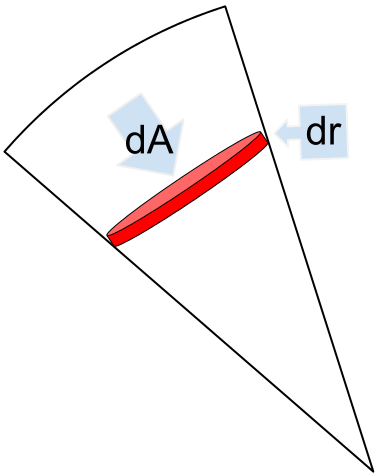
\includegraphics[totalheight=4cm]{plot/wd1}
\caption{How could be infinitesimal fluid element laying between 
$r$ and $r+\mathrm{d}r$ with an area $\mathrm{d}A$ imagine}
\label{wd1} 
\end{figure}

The gravitation attraction between mass $\mathrm{d}m = \rho \mathrm{d}A \mathrm{d}r$ and $m(r)$ is the same as if $m(r)$ were only point at the center with the same mass. While the outside mass exerts no force on $dm$.
Then the net outward pressure forced on $\mathrm{d}m$ is $- \left [ P\left ( r + \mathrm{d}r \right ) - p(r)  \right ]\mathrm{d}A$. In equilibrium 
\begin{equation}
\label{eq1}
 \frac{\mathrm{d}P}{\mathrm{d}r} = - \frac{Gm_{(r)}\rho}{r^2}
\end{equation}
In such equilibrium, the gradient of degeneracy pressure is balanced by gravitation: 
\begin{equation}
\label{equ_1}
\nabla P = -\rho \nabla \Phi, 
\end{equation}
where $\Phi$ means gravitation potential.  
Consequence of the Eq.\eqref{eq1} is the viral theorem. The gravitation potential energy of the star is then 
\begin{equation}
\label{pot_e_star1}
W = -\int_{0}^{R} \frac{Gm(r)}{r}\rho 4 \pi r^2 \mathrm{d}r = \int_{0}^{R} \frac{\mathrm{d}P}{\mathrm{d}r}4\pi r^3 \mathrm{d}r = -3\int_{0}^{R} P4 \pi r^2 \mathrm{d}r
\end{equation}
We can characterize the gas by an adiabatic equation of state, where $K$ and $\Gamma$ are constants
\begin{equation}
 \label{adiab_1}
P = K\rho_0^\Gamma
\end{equation}
Then Eq.\eqref{pot_e_star1} can be rewritten as follows
\begin{equation}
 W = -3 (\Gamma - 1) U,
\end{equation}
Where $U$ is the total star's internal energy 
\begin{equation}
U = \int_{0}^{R}\varepsilon' 4\pi r^2 \mathrm{d}r 
\end{equation}
and $\varepsilon'$ comes from:
\begin{equation}
\label{eps1}
 \varepsilon' \equiv \varepsilon - \rho_0 c^2
\end{equation}
where
\begin{equation}
 \varepsilon = \rho_0c^2+\frac{P}{\Gamma -1}
\end{equation}
Now we can see that the energy density, of the gas (excluding the rest mass energy) can be also written as
\begin{equation}
 \label{eps2}
 \varepsilon'=\frac{P}{\Gamma - 1}
\end{equation}
Assuming adiabatic changes, the Eq.\eqref{eps2} follows from the first law of thermodynamics
\begin{equation}
 \mathrm{d}\left ( \frac{\varepsilon }{\rho_0} \right ) = -P\mathrm{d}\left ( \frac{1}{\rho_0} \right ) .
\end{equation}

The equation of state for ideal Fermi gas reduce to the simple polytropic form Eq.\eqref{adiab_1} in
the two limiting cases \citet{2004bhwd.book.....S}, \citet{padm_vII}:
\begin{itemize}
\item Nonrelativistic electrons, $\rho_0 \ll 10^6 g.cm^{-3}, x\ll 1, \Phi_{(x)}\rightarrow x^5/15\pi^5 $
\begin{equation}
\Gamma = \frac{5}{3} \Longrightarrow  K = \frac{3^{2/3}\pi^{4/3}}{5}\frac{\hbar^2}{m_em_u^{5/3}u_e^{5/3}} = \frac{1.0036\times 10^{13}}{u_e^{5/3}} \mathrm{cgs}.
\end{equation}
\item Extremly relativistic electrons, $\rho_0 \gg 10^6 g.cm^{-3}, x\gg 1, \Phi_{(x)}\rightarrow x^4/12\pi^2 $
\begin{equation}
\Gamma = \frac{4}{3} \Longrightarrow K = \frac{3^{1/3}\pi^{2/3}}{4}\frac{\hbar c}{m_u^{4/3}u_e^{4/3}} = \frac{1.2435\times 10^{15}}{u_e^{4/3}} \mathrm{cgs}.
\end{equation}
\end{itemize}

This kind of the equilibrium configurations such these are called polytropes. We can use Eq.\eqref{equ_1}, take the divergence of it and by using $\nabla^2\Phi = 4\pi G \rho$ in spehrically 
symmetric case we get  
\begin{equation}
\label{pol_1}
 \frac{1}{r^2}\frac{\mathrm{d}}{\mathrm{d}r}\left ( \frac{r^2}{\rho}\frac{\mathrm{d}P}{\mathrm{d}r} \right ) = -4\pi G\rho .
\end{equation}
Using few trics, Eq.\eqref{pol_1} can be rewrite and reduce to dimension less form 
\begin{equation}
 \label{pol_2}
\frac{1}{\xi^2 }\frac{\mathrm{d}}{\mathrm{d}\xi}\xi^2\frac{\mathrm{d}\theta }{\mathrm{d}\xi } = -\theta^n 
\end{equation}



use Eq.\eqref{adiab_1} with $\Gamma \equiv 1 + \frac{1}{n}$ where $n$ is called the polytropic index
\begin{equation}
\label{pol_3}
\rho = \rho_c \theta^n  
\end{equation}
\begin{equation}
\label{pol_4}
r = a\xi
\end{equation}
\begin{equation}
\label{pol_5} 
a = \left [ \frac{\left ( n+1 \right ) K \rho_c^{\left ( 1/n-1 \right )} }{4\pi G} \right ]^{1/2}
\end{equation}
where $\rho_c$ is the central density, $\rho_c = \rho$ when $r = 0$. 

The Eq.\eqref{pol_2} is called the \textit{Lane-Emden equation} for the structure of $n$ index, the boundary 
conditions at the center such polytropic white dwarf are
\begin{equation}
\label{le1}
 \theta(0) = 1, 
\end{equation}
\begin{equation}
\label{le0}
 \theta'(0)= 0.
\end{equation}
The condition \eqref{le1} come dirrectly from Eq.\eqref{pol_3} and condition \eqref{le0} is derived from the fact 
that near the center of the star is $m(r) \approx 4\pi \rho_c (r^3/3)$. If we use Eq.\eqref{eq1}, we get
\begin{equation}
 \frac{\mathrm{d}P_{(\rho)}}{\mathrm{d}r} = \frac{\mathrm{d}\rho}{\mathrm{d}r} = 0 .
\end{equation}

If we numerically integrate Eq.\eqref{pol_2} using Eq.\eqref{le1} and Eq. \eqref{le0} as the boundary conditions, 
starting at $\xi=0$. We will find that for $n<5$ $(\Gamma>6/5)$ this solution decrease monotonically with a zero 
at finite value $\theta(\xi_1) = 0$, which corresponds to the star's surface where $P=\rho = 0$ and we get the 
equation for white dwarf radius 
\begin{equation}
 \label{radius1}
R = a\xi_1 = \left[ \frac{(n+1)K}{4\pi G} \right]^{1/2}\rho_c^{\frac{1-n}{2n}}\xi_1.
\end{equation}

The mass of the WD can be find as follows
\begin{equation}
 \label{wdmass}
\begin{split}
M &= \int_{0}^{R} 4\pi r^2 \rho \mathrm{d}r \\
  &= 4 \pi a^3 \rho_c \int_{0}^{\xi_1} \xi^2 \theta^n \mathrm{d}\xi \\
  &= -4 \pi a^3 \rho_c \int_{0}^{\xi_1}\frac{\mathrm{d}}{\mathrm{d}\xi}\left( \xi^2 \frac{\mathrm{d}\theta}{\mathrm{d}\xi}\right)\mathrm{d}\xi \\
  &= 4 \pi a^3 \rho_c \xi_1^2 \lvert \theta' (\xi_1) \lvert \\
  & = 4 \pi \left[ \frac{(n+1)K}{4 \pi G}\right]^{3/2} \rho_c^{\frac{(3-n)}{2\pi}}\xi_1^2 \lvert \theta' (\xi_1)\lvert ,
\end{split}
\end{equation}
then $\rho_c$ can by eliminated between Eq.\eqref{radius1} and Eq.\eqref{wdmass}, which gives the mass-radius relations 
for polytropes \citet{2004bhwd.book.....S}:  
\begin{equation}
\label{mr_eq}
 M = 4 \pi R^{\frac{3-n}{t-n}}\left[ \frac{(n+1)K}{4 \pi G}\right]^{\frac{n}{n-1}}
\xi_1^{\frac{3-n}{1-n}}\xi_1^2\lvert\theta' (\xi_1) \lvert \: .
\end{equation}

\section{The Chandrasekhar limit}
What will happen if $\rho_c \rightarrow \infty$? This is one of the most important questions in the universe. 
Because how central density of WD increases by increase of the WD mass, the electrons become more and more 
relativistic throughout the star. As $R\rightarrow 0 $ also the space for free electrons moving between atoms nuclei become
smaller and smaller. With increasing mass must also increase the speed of electrons to support the degeneracy pressure.  
While the mass of WD is larger the radius become smaller, mass-volume relations implies that $\rho\propto M_{WD}^2$. 
But the electrons can't have speed larger than speed of light and in some point where $\rho \sim 10^9 \mathrm{g\:cm^{-3}}$ there 
will be no space left for moving electrons and they will be press into the nuclei. This will leads to explosion of such WD. 

\begin{figure}[hbt!]
\centering
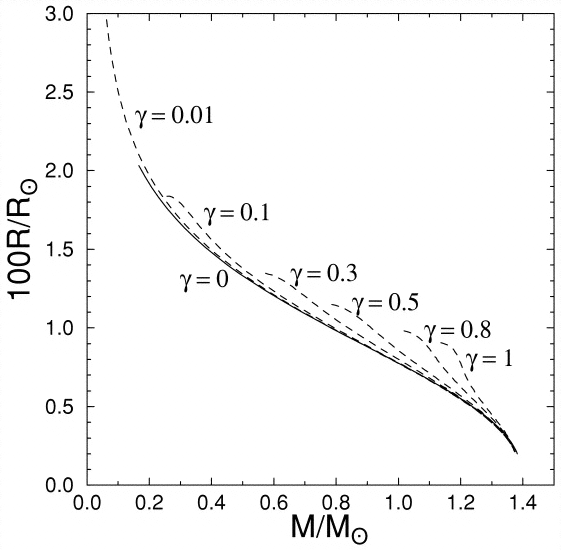
\includegraphics[totalheight=8cm]{plot/chlimit}
\caption{Relation between the mass $M$ and radius $R$ of a $^{12}C$ magnetic white dwarf for the indicated magnetic field strengths. 
The solid line denotes the \citet{1961ApJ...134..683H} model for nonmagnetic white dwarfs $(\gamma = 0)$. The dashed lines are magnetic 
white dwarfs. \citet{2000ApJ...530..949S} }
\label{Chlimit1} 
\end{figure}

This all means, that there is a maximum mass for WDs. This mass is called \textit{Chandrasekhar limit}
\footnote{Named after Indian physicist Subrahmanyan Chandrasekhar who received the Nobel Price in Physics in 1983 for his 
work on stellar structure and evolution. Chandrasekhar made his great discovery at the age of 21 in the 1931.   } $M_{ch}$.  

The classical theory of type 1A supernovae assumes explosions of such WDs reaching the $M_{ch}$, the very same 
mass of the WDs when they explode makes Type 1A supernovae perfectly suitable objects for measuring the long range 
space distances. That's why they are so important objects for cosmology and astronomers called 
them standard candles.

The Chandrasekhar limit for relativistic electron case is
\begin{equation}
 \label{chlim}
M_{ch}=1.457\left ( \frac{2}{\mu_e} \right )^2 \mathrm{M_{\odot}} \:,
\end{equation}
where $\mu_e$ is the average molecular weight per electron, which depends on the chemical comsposition of the star and is typically sets 
to $\mu_e = 2$. 

The Eq.\eqref{chlim} can be obtained by solving Eq.\eqref{mr_eq} with parameters\footnote{Extensive list of polytropic parameters can be find in
\citet{1939MNRAS..99..673C}}:
\begin{equation}
\Gamma = \frac{4}{3}\:,\:\: n =3 \:,\:\: \xi_1 = 6.89685 \:,\:\: \xi_1^2 \lvert \theta' (\xi_1) \lvert = 2.01824\:\:. 
\end{equation}
                                                                                                                                                                                                                                                                                                                                                                                                                                                                                                                                                                                                                                                                                                                                                                                                                                                                                                                                                                                                                                                                                                                                                                                                                                                                                                                                                                                                                                                                                                                                                                                                                                                                                                                                                                                                                                                                                                                                                                                                                                                                                                                                                                                                                                                                                                                                                                                                                                                                                                                                                                                                                                                                                                                                                                                                                                                                                                                                                                                                                                                                                                                                                                                                                                                                                                                                                                                                                                                                                                                                                                                                                                                                                                                                                                                                                                                                                                                                                                                                                                                                                                                                                                                                                                                                                                                                                                                                                                                                                                                                                                                                                                                                                                                                                                                                                                            
Another, ilustrativ aproach to estimating the Chandrasekhar limit is mention in \citet{2007ima..book.....C}. An approximate value for $\mathrm{M_{ch}}$ may by 
obtain by setting the estimate of the central pressure
\begin{equation}
 P_c \approx \frac{2}{3} \pi G \rho^2 R_{wd}^2 \qquad \text{with} \qquad \rho=M_{wd} / \frac{4}{3} \pi R_{wd}^3  
\end{equation}
equal to electron degeneracy pressure equation
\begin{equation}
 \label{edegP}
P = \frac{(3\pi^2)^{2/3}}{4} \hbar c \left[ \left( \frac{Z}{A}\right) \frac{\rho}{m_H}\right]^{4/3},
\end{equation}
with $Z/A=0.5$, the $R$ cancels from the equation leving for the greatest possible mass:
\begin{equation}
 \label{chlim2}
M_{ch} \sim \frac{3\sqrt{2\pi}}{8}\left ( \frac{\hbar c}{G} \right )^{3/2}\left [ \left ( \frac{Z}{A} \right ) \frac{1}{m_H} \right ]^2 M_\odot.  
\end{equation}
It is important to notice that Eq.\eqref{chlim2} contains three fundamental constants $\hbar, c$ and $G$ representing the combined effects of quantum mechanics, 
relativity and Newtonian gravitation on the WD structure. 

The Chandrasekhar limit slightly depends upon the chemical composition \eqref{chlim}, but in the literature is well known as $M_{ch} = 1.44M_\odot$.    
  
The similar limit exists for neutron stars, where pressure of degenerate neutron gas support the stars against it own gravity. 
This limit is called Tolman --- Oppenheimer --- Volkoff limit (or TOV limit).But it is not so easy in neutron stars case. Their limit 
mass depends strongly on type of matter in star center. The limit varies from $0.7 M_\odot$ up to $\sim 3M_\odot$ in extreme case, when inner section of 
neutron star is partialy filled up by quark - gluon matter.     


\section{White dwarfs classes}
Previous sections describe interior and fundamental parameters of white dwarfs, but it also important to tell something about their classes.   
WDs occupy narrow sliver line in the left bottom corner of H-R diagram fig.(\ref{hrd1}), slightly parallel with the main sequence.  
Although WDs are typically whiter then normal stars, the name itself is not very comprehensive. WD in fact come in all colors with surface 
temperatures from less than $4000K$ to even more than $80,000K$. The $D$ for \textit{dwarf} spectral type has several subdivisions:
\begin{itemize}
 \item \textbf{DA} white dwarfs is the largest group $(\sim 60\%)$ including Sirius B, their spectra have only pressure-broadened hydrogen lines 
 \item \textbf{DB} white dwarfs $(\sim 8\%)$ have only helium absorbtion lines in their spectra 
 \item \textbf{DC} white dwarfs $(\sim 14\%)$ have no lines, but only continuum features
 \item \textbf{DQ} white dwarfs show carbon features in their spectra
 \item \textbf{DZ} white dwarfs show some evidence of metal lines
\end{itemize}

Very small radius makes WDs hard to observed in optical band. The brightest and also the most known WD is Sirius B with visual magnitude $\sim8.6$. 
Unfortunately it is located only $8”$ from his companion Sirius A, the brightness star of the night sky. Although the WD are not common stars 
on the  night sky, their are not rare in our Galaxy. From hundred closes stars to our Sun, eight of them are WDs.

WDs usually have very strong magnetic field which comes from weak surface magnetic field of progenitor's star which lagre surface are conserved to their very 
small surfaces. The magnetic field intensities vary from about $1000 \:\mathrm{G}$ up to $10^9 \:\mathrm{G}$ in extreme cases.    

WDs can by find alone in interstellar space, young ones can be find also in planetary nebulae, like one  in center of the Ring nebula 
M57 or their can be find in cataclysmic variables.       
 
\begin{figure}[hbt!]
\centering
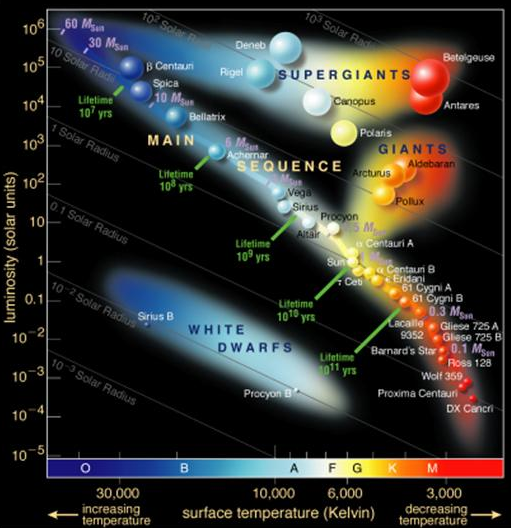
\includegraphics[totalheight=12cm]{hrdiagram}
\caption{WD lies in right bottom corner of HD diagram, under main 
sequence, which exactly means, they are very small (dwarf) stars with high surface temperature.  }
\label{hrd1} 
\end{figure}


\chapter{Cataclysmic variable stars}

Cataclysmic variable stars \textit{(CVs)} received their name for their cataclysmic events, like outbursts, novae and supernovae eruptions. 
In this one name several very different mechanisms are used for creating the various cataclysmic events.         
Dwarf novae are common for their increase of brightness by factor ten, classical novae are increasing their 
brightness usually in factor $10^6$ and type 1A supernovae in factor $10^{12}$, typical visual absolute magnitude 
for them is $M_V = -19.3$\footnote{About $5\times10^9$ times brighter than the Sun}.  

What is common for all the CVs types is their binary star character with mass transfer through Roche lobe to primary 
companion, which is white dwarf star. Several thousands of CVs with even more candidates are known up to date. 
The mean mass of the primary star is $\sim 0.8 M_\odot$, which is larger than the average of $\sim 0.6 M_\odot$ for isolated, 
forever alone WDs.
The secondary star is a main-sequence low mass star of G or later type, but usualy with less mass then the primary WD.      

Configuration like this make stars orbit each other with periods from around 20 minutes up to several days, 
however the vast majority of CVs have orbital periods from $1$ to $12$ hours\footnote{Interesting think is that there exists a "period gap" 
in CVs periods in range from 1.5 to 3.25 hours. The cause of this gap is not well understood yet. }.

The various classifications and approaches to study the CVs exists. They mostly depends on the different wavelength in which the CVs are 
observed. The biggest and also the well observed is optical band where we can see these types: 
\begin{itemize}
 \item \textbf{Classical novae} are characterize by large outbursts couses by thermonucler exlosion of accreted material on WD's surface
 \item \textbf{Recurrent novae} have small outbursts repeating every few years, typical example is RS Oph
 \item \textbf{DN - dwarf novae} use to have several smaller outbursts, have several subclases \textit{(Z Cam, SU UMa, SS Cyg\footnote{SS Cygni had few 
outbursts, but according to latest obervations, it seems to be more-likely intermediate polar})} 
 \item \textbf{AM Canum Venaticorum} are extremely interesting space objects where the secondary star is also a compact object and the accretion 
disk is mostly composed from helium and they could by source of strong gravitation waves 
 \item \textbf{Novae like systems} are possible nova remnants or stars with outburst behavior similar to novae but maybe miss-classify
 \item \textbf{Polars} are magnetic CVs with $B \sim 10^7 - 10^9 \:\mathrm{G}$, they got the name because of strong polarization of their light in optical and IR bands 
 \item \textbf{IP intermediate polars} are magnetic CVs with $B$ less then polars $\sim10^6-10^7\: \mathrm{G}$ 
 \item \textbf{Type 1A supernova} is sub-class of supernovae which become a result of thermonuclear explosion of whole WD when it reaches the $M_{ch}$ limit  
\end{itemize}

During last years CVs became more and more attractive target for modern astronomers mainly because of  
the progress in detectors technology in different then optical band and also for their role as a 
space laboratories for study accretion of matter on compact star, X-ray emission from shock regions, 
and even gravitation waves. 

The CVs are complex and complicated space objects, for this reason is hard to make a good 
classification. If we look inside \citet{warner:1}, we will find several fact which are not 
consider as correct now. With new huge sky surveys as GAIA\footnote{Is space mission
to chart a three-dimensional map of our Galaxy, will observed $\sim$ one billion stars. Launch is planned for 2013.} 
or LSST\footnote{The Large Synoptic Survey Telescope (LSST) will be wide-field survey $8.4\: \mathrm{m}$ 
telescope which will photograph the available sky every three nights from his place on the 
El Peñón peak of Cerro Pachón, at 2682 m in Chile. } the new and even more 
complex classification will need to take place.    
The number of known CVs systems will grow rapidly, also as the number of observations. Next decade 
will be the gold era for new scientific approaches like data-mining in huge amount of data-sets.

In following sections of this work we use the most broad CVs classification, for magnetic and non-magnetic
systems. Because of the aim of this work on magnetic systems, we will take care of non-magnetic only  
roughly. Please also note, that if we want to make a very good classification of CVs to many classes, 
almost everyone of them will has its own class.  


  
\section{Non magnetic cataclysmic variables} 
The magnetic field plays essential role in all the CVs, even in non-magnetic ones, at-least weak 
magnetic field provides viscosity in accretion disk. We will called non-magnetic CVs when 
$B\lesssim10^5 \: \mathrm{m}$. 
In such system is movement of gas from the secondary companion to the WD determined predominantly 
by dynamical and hydro-dynamical flows \citet{warner:1}.

\begin{figure}[hbt]
\centering
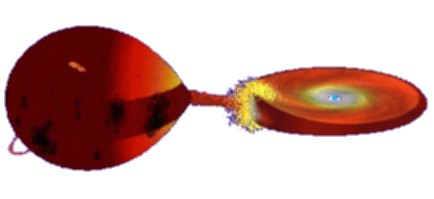
\includegraphics[totalheight=3cm]{plot/cv}
\caption{The illustration of cataclysmic variable star, showing the normal, secondary star on the right, accretion stream meeting 
the accretion disk and accretion disk itself around the white dwarf. }
\label{cv1} 
\end{figure}

The non-magnetic CV could looks like fig.\ref{cv1} or the \textit{(A)} part of fig.\ref{all_typescv}. The secondary is a small main sequence star with mass about 
half of the Sun mass which is filling out its Roche lobe. The mass transfers from secondary to primary
through the Lagrangian point L1 and in some point its creates the accretion disk. Streaming mass meets the accretion disk and if the mass stream is big enough and disk is dense enough, so called 
hot spot is created as we can see on fig.\ref{cv1}.  

\subsection{Orbital periods}
Orbital period $P_{orb}$ is usually the most precisely know physical parameter of CV. Because of facts that the 
CVs orbital periods are relatively short and to take enough data-sets to create a phase light curve 
is then not that difficult task. $P_{orb}$ of the system reveals how big the CV systems are. The most of the 
CVs with typical periods in range hours can fit inside Earth - Moon orbit. 

Inspecting the Riter \& Kolb catalogue \citet{2003A&A...404..301R} within the orbital period range from 1 hour to 1 day, without the AM CVn systems, 
it is found that almost half of all CVs in catalogue are the dwarf novae.
\begin{itemize}
 \item 166 DNs $63\%$ have $P_{orb} < 2h$
 \item 26 DNs $10\%$ are found in the 2-3 h gap 
 \item 70 DNs $27\%$ are behind the gap with $P_{orb} > 3h$  
\end{itemize}
The conventional idea about where the gap comes from points to internal structure changing in the secondaries.   
In some point of secondary star evolution it has a radius corresponds to its mass in excess of the equilibrium value. 
This force secondary to detaches  from Roche lobe foe a while. The stellar wind is also very low during this period which cause disappearance of accretion disk.
The period gap and the orbital period distribution per all the CVs and between the different CVs types is well shown on fig.\ref{cv_orb1}.  

\begin{figure}[hbt!]
\centering
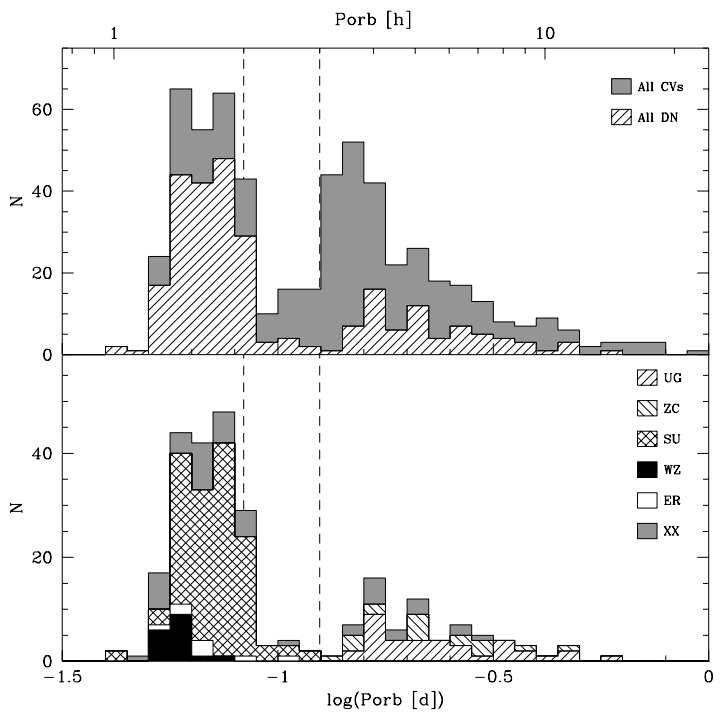
\includegraphics[totalheight=12.5cm]{plot/cv_orbper.png}
\caption{\textit{Top panel}: the orbital period distribution of known CVs and dwarf novae from are shown in gray and 
shade \citet{2003A&A...404..301R}. \textit{Bottom panel}: the period distribution of known dwarf novae according to their subtypes, U Gem (UG), 
Z Cam (ZC), SU UMa (SU), WZ Sge (WZ), ER UMa (ER), and unclassified subtype (XX). The dashed lines represent the conventional 
2-3h period gap \citet{Aungwerojwit}.}
\label{cv_orb1} 
\end{figure}

\section{Magnetic cataclysmic variables}
Magnetic CVs are these where the strong magnetic field significantly affects the accretion process. These systems are divided 
according to strength of their magnetic field to two categories: 
\begin{itemize}
 \item Polars, also called AM Herculis stars, $B_{wd} \sim 10^7 - 10^9\: \mathrm{G}$  
 \item Intermediate polars $B_{wd} \sim 10^6 - 10^7 \: \mathrm{G}$
\end{itemize}


\begin{figure}[hbt!]
\centering
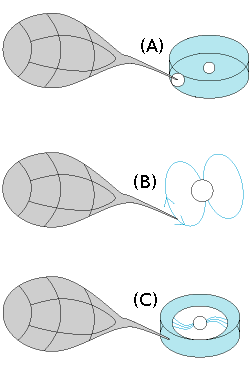
\includegraphics[totalheight=5cm]{plot/binall}
\caption{An illustration of difference between non-magnetic and magnetic CVs. \textit{(A)} is an illustration of non-magnetic 
disk-type system, same as artist impression fig.\ref{cv1}. \textit{(B)} is a system with strongly magnetized WD called Polar 
where magnetic field prevent creations of accretion disk and the in-falling material forms an accretion stream following the 
magnetic field lines of WD.
\textit{(C)} is intermediate case between \textit{(A)} and \textit{(B)}, the not such strongly magnetized WD as one in polars 
destroying only inner part of accretion disk by his $B_{wd}$ creating accretion curtain following its magnetic field lines. }
\label{all_typescv} 
\end{figure}

\subsection{Polars}
The \textit{(B)} part of fig.\ref{all_typescv} is how schematically polars looks like. The material from secondary is falling via 
the inner Lagrangian point towards to the primary, which is the highly magnetized WD as was mention before. The gas in the
 stream is ionized by collisions and X-rays from the accretion region on the WD. In some point at the stream's trajectory 
the magnetic energy density of the WD's field is sufficient to divert the stream from its free fall trajectory and force 
it to follow the magnetic field lines. Accretion therefore occurs over a small area near both or one of the magnetic poles 
of the WD. The magnetic field is assumed to be bipolar \citet{1990SSRv...54..195C}.

How material traveling at roughly the escape velocity of the WD it approaches to the surface of the WD a very strong shock 
region is formed in accretion flow. The hard X-rays are emitted from post-shock region. Fraction of X-rays is reprocessed 
by the surface of WD and re-emitted as the softer X-rays component. 

Free electrons close to the shock spiral around the magnetic field lines, therefore, emit strongly polarized 
cyclotron radiation. The magnetic field of WD is such strength that the cyclotron radiation is emitted in optical and 
near infra-red wavelengths.               

In polars, the WD magnetic field is sufficiently strong to force the primary to rotate synchronously. The magnetic field 
therefore always present the same section to the incoming accretion stream. This is the principal distinguishing feature 
for polars (intermediate polars rotates asynchronous).   

The principal defining characteristic of the polar CVs class is their strongly and variably circularly 
and linearly polarized optical emission. They are also characterized by high ratio of soft-to-hard X-ray 
luminosity and high excitation optical spectra with prominent He II 468.6 emission lines. For a review of the polars, see \citet{1990SSRv...54..195C}
or \citet{warner:1}.  

\subsection{Intermediate polars}
%\section{Galactic population of the cataclysmic variables}
%\section{GXRE}
The \textit{(C)} part of fig.\ref{all_typescv} illustrates how can be intermediate polars imagined. 
They are CVs with not as strong magnetized WDs as in polars. This is causing a several important 
differences between polars and IPs. In IPs the other part of accretion disk exists, but at some 
distance of WD the kinetic energy density $\rho v^2$ of gas in accretion disk is locally exceeded by the
 magnetic energy density $B^2/8\pi$ and within this radius the in-falling gas will be guided along magnetic 
field lines to accrete radially onto the WD creating kind of accretion curtain.  
For the spherical accretion is easy to calculate transition radius, because $v$ is simply the 
free-fall velocity: $\sqrt{2MG/r}$, the radius is according \citet{1994PASP..106..209P}:
\begin{equation}
\label{ipra}
R_A = 3.7 \times 10^9 \dot{M}_{1}^{-2/7}M_{wd}^{-1/7}\mu_{32}^{4/7} \mathrm{cm},
\end{equation}
where $R_A$ is the \textit{Alfven radius}, $\dot{M}_{1}$ is the accretion rate in 
units of $10^{17}\:\mathrm{g\:s^{-1}}$, $M_{wd}$ is the mass of WD in units $\mathrm{M_\odot}$ and $\mu_{32}$ is the magnetic moment 
of the WD in units of $10^{32}\:\mathrm{G\:cm^3}$. For disk accretion, the magnetospheric radius should be slightly 
smaller, theoretical estimates suggest $R_{mag} \approx 0.5R_A$ \citet{1994PASP..106..209P}.  

As the gas almost freely fals onto WD channeled along magnetic field lines, in some distance near the 
WD surface a stationary shock stands to convert the kinetic energy of the gas into thermal energy, 
\citet{2010A&A...520A..25Y}.
The temperature of such shock heated gas is typically over 10keV and the density is low. The hard X-rays 
are emitted via optically thin thermal emission. Then the heated gas forms a post shock region (PSR) 
with a temperature gradient. The gas descends while it is cooled via X-ray emission and finally hits 
the surface of WD with small energy by emitting UV light \citet{1973PThPh..49.1184A_aizu}. 
This property makes from IPs very good targets for hard X-ray space missions. The closer look to PSR 
will be taken in the next chapter.   

\begin{figure}[hbt]
\centering
\includegraphics[totalheight=12cm]{plot/bb_spec_cv_krivonos}
\caption{Typical broadband spectra of different CVs' classes, indicating that INTEGRAL observations in 
the hard X-ray energy band (17--60 keV) are biased toward detecting the hardest CVs -- intermediate polars, 
\citet{2008A&A...489.1121R}.}
\label{kriv_1} 
\end{figure}


\chapter{Masses of white dwarfs in intermediate polars}
As it was mentioned before, the mass of a WD is the most fundamental parameter in CVs. It is also the 
main parameter characterizing the accretion flow, the emission from the accretion region and, most 
importantly, it is the parameter which governs the dynamics of orbital motion of the system. The 
knowledge of WDs' masses in CVs plays a fundamental role in understanding the binary evolution. 

Previous attempts to determine the WDs' masses in IPs using X-ray measurements did not succeed, 
because the data from different instruments led to different mass estimates. In all cases, the 
masses  determined by the X-ray measurements where substantially higher than masses derived from  the optical 
observations. The most notable example is XY Ari, which is an eclipsing IP with a very small uncertainty in 
the inclination (\citet{1998MNRAS.297.1269R}).          
\begin{itemize}
 \item RXTE spectrum yields 1.22 M$_\odot$
 \item ASCA data yields 1.27 -- 1.4 M$_\odot$
 \item Ginga results 1.3 M$_\odot$
 \item the optical methods yields 0.78 -- 1.03 M$_\odot$ 
\end{itemize}
Observations in hard X-rays over 20 KeV are crucial as they provide a clean signal, not contaminated 
by other system components such as the accretion disc or the main-sequence star and they avoid 
complications due to cold or warm absorbents as well as the fluorescence emission (\citet{2009A&A...496..121B}). 
However, this method is not suitable because of the weakness of the X-ray flux. In spite of the fact that the IPs 
are among the brighter sources in the hard X-ray sky, their photon count is relatively low. Thus a sensitive 
instrument must be used for this kind of observations. At present, there are three instruments which are 
widely used for such observations: Swift/NASA Burst Alert Telescope, Hard X-ray Detector
(HXD) on-board Suzaku/JAXA space mission and IBIS on-board INTEGRAL/ESA.

The idea how to study the post-shock region, the X-ray emission from IPs and then 
determine the mass of WD is to try to cover broad bands from soft to hard X-rays. Ideally, 
from 1keV up to 100 keV. In the softer X-rays below 10 keV there are, however, several other features 
present, but the photon flux in this band is much higher than in bands over 15 keV. 

In this case, it is necessary to combine two different detectors, one for soft and one 
for hard X-rays. The optimal combination would be XMM-Newton for soft X-ray in range 1–10 keV 
and INTEGRAL for hard X-ray from 20–100 keV. 

This combination provides a good compromise. The photon flux in the soft X-ray is high enough 
to allow short pointings of XMM with a good s/n ratio. However, the fitting model for such spectrum 
can be complicated because of the presence of several other features e.g. reflections or the 6.4 keV 
emission line.

The hard X-rays are important for the localization of the spectral energy cut-off so a good fit 
of the model, either power-law or bremsstrahlung, can be applied. INTEGRAL/IBIS is, 
due to a relatively good sensitivity and large field of view (FOV), a suitable instrument 
for observations in this band. The large FOV allows a good coverage 
of the X-ray sky enabling long exposures covering multiple objects in this band.  

\section{Post shock region}
Reason why IPs are the most suitable for measurements of the mass of their WD companion then others CVs 
is their magnetic field, which is not as low as in non-magnetic CVs $B<10^6$ but still weaker then in 
polars $B\gtrsim10^7$. 
As was mentioned before, in IPs is the accretion disk destroyed in some distance from WD and accretion 
continues through accretion curtain, where the gas follows magnetic force lines. 
The resulting configuration is often know as an accretion column. 
From theory of spherical accretion (\citet{accpower:1}) we expect that accreting matter to be highly 
supersonic and therefore in free-fall above the WD's pole-caps. 

The in-falling matter must be somehow decelerated to subsonic velocities in order to accrete, 
therefore we expect strong shock-wave in matter stream where the kinetic energy of infall 
\begin{equation}
\frac{1}{2}\upsilon_{ff}^2 = GM_{wd}/R_{wd}, 
\end{equation}
will be turned into thermal energy. Because that $m_p \gg m_e$ the ions are these who brings the most of this kinetic energy supply. 
The kinetic energy of ions must by emitted, absorbed or re-emitted by WD. The luminosity corresponding 
to the typical accretion rate $\dot{M} \gtrsim 10^{16} \mathrm{g\:s^{-1}}$ will be of order 
$10^{33} \mathrm{erg\:s^{-1}}$ which greatly exceed any intrinsic luminosity (typically 
$\ll 10^{31} \mathrm{erg\:s^{-1}}$) that the WD may have as a result of left-over thermal energy in its 
degenerated core (\citet{accpower:1}).  

The accretion luminosity is according to \citet{accpower:1}:
\begin{equation}
\label{lacc}
L_{acc} \lesssim 2 \times 10^{29}f_{-2}m_1^{18/7}R^{-1/7} \: \mathrm{erg \: s^{-1}},
\end{equation}
where $f_{-2} = 10^2 f$ and $f$ is a surface fraction.Which is much lower then the bolometric luminosities 
of observed CVs. Therefore, we must conclude that the infaling matter goes through strong shock which 
slows it down before reaching the WD surface.    

Now we know that the shock gas is hot with characteristic (shock) temperature
\begin{equation}
\label{br_ts}
 T_s = \frac{3}{8}\frac{G M \mu m_H}{k R_{wd}}=3.7 \times 10^8 m_1 R^{-1} \mathrm{K}. 
\end{equation}

From previous chapters we already know that the main cooling mechanism is thermal bremsstrahlung, but 
lets try to determine this on our own a little bit. 

In steady state in accretion column, the accretion energy released below the shock must be removed 
from the post-shock column at the same rate in which it is deposited. Such removal must be effected 
by a combination of the cooling mechanisms such as radiation and particle transport processes. It is also 
determined by distance of the shock-wave from WD surface. 

If the cooling were inadequate the gas in PSR would simply expand adiabatically and raise 
the shock. On the other hand, if cooling became too effective the shock would move in towards the 
WD surface, reducing the volume of the PSR cooling region (\citet{accpower:1}).  

\begin{figure}[hbt]
\centering
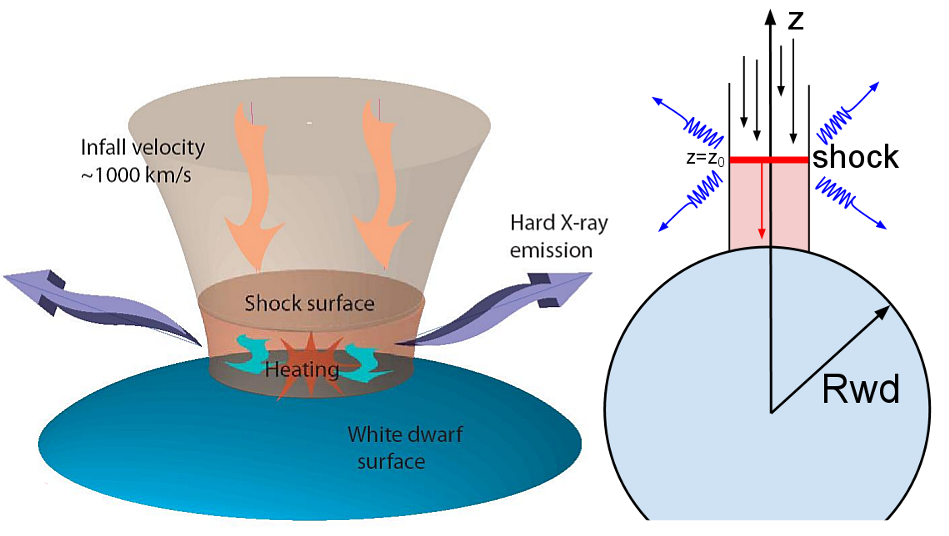
\includegraphics[totalheight=5cm]{plot/psr2}
\caption{Both images are showing the same accretion column geometry for a IP. The shown accretion column 
is circular and accretion plasma is assume to be uniform across the column, image is from the \citet{krivonos_pres}. 
\textit{The left} figure is showing
3D illustration while \textit{the right} one shows the schematically the geometry of the PSR.}
\label{psr1} 
\end{figure}

For understanding and constructing appropriate accretion column model we must specify how the shock-heated 
gas in PSR is cooled. The estimation of which cooling mechanisms is important in IPs should be based on 
following ideas. 

The gas velocity below the shock is according to \cite{accpower:1} 
\begin{equation}
\upsilon = 1.3 \times 10^8 m_1^{1/2}R^{-1/2} \mathrm{cm \: s^{-1}}, 
\end{equation}
using the continuity equation 
\begin{equation}
 4\pi R^2 f(- \rho \upsilon) = \dot{M}
\end{equation}
we can find a PSR gas density corresponding to the electron density
\begin{equation}
 \label{gas_el_den_PSR}
\begin{split}
\rho_{PSR} &= 6.2 \times 10^{-10} \dot{M}f_{-2}^{-1}m_1^{-1/2}R^{-3/2} \: \mathrm{g \: cm^{-2}} \:, \\
N_e &= 5.9 \times 10^{14} \dot{M} f_{-2}^{-1}m_1^{-1/2}R^{-3/2} \: \mathrm{cm^{-3}} \:, 
\end{split}
\end{equation}
assuming a fully ionized gas with standard cosmic abundance. 
With characteristic PSR gas temperature $T_s$ is electron scattering only possible source of opacity. 
The shock distance from WD surface is lower the $R_{wd}$. The results of this is that the horizontal optical 
depth is relatively low, therefore the radiative cooling will be optically thin (unless the accretion 
rate per unit area will be extremely high).   
  
Because of high $T_s$ (Eq.\eqref{br_ts}), radiative cooling of the PSR gas will be dominated by the 
bremsstrahlung (free—free) emission. The volume emissivity is
\begin{equation}
4\pi j_{bremss} \cong 2 \times 10^{-27} N_e^2 T_e^{1/2} \mathrm{erg \:s^{-1} \: cm^{-3}}, 
\end{equation}
for a gas of cosmic abundance with electron temperature and density $T_e$, $N_e$.  

The estimates from last paragraphs show that the PSR is hot, optically thin and that shock lies quite 
close to the WD surface. The falling gas is cooled by optically thin bremsstrahlung emission and then 
it hits WD surface, with much lower than free-fall speed, where black-body emission will take place 
with maximum in UV band.   

We may briefly consider some of the extreme cases. If the WD is extremely massive close to the $M_{ch}$ 
therefore with very low $R_{wd}$ and the accretion stream will be low, the Compton scattering will 
become important as radiative cooling process. Also the cyclotron cooling, which is negligible in 
IPs, will take place in case of low accretion stream and higher $B_{wd}$.   

\subsection{Bremsstrahlung}
Bremsstrahlung is a German word for breaking radiations, which is a radiations due to the acceleration 
of a charge in the Coulomb field of another charge also called as free-free emission. A full 
understanding of this process requires a quantum treatment, since photons of energies comparable 
to that of the emitting particle can be produced, \citet{rybicki:1}.

The electrostatic accelerations of the in its rest frame, parallel $a_{\parallel}$ and perpendicular 
$a_\perp$ to its direction of motion are:        
\begin{equation}
\label{brem1}
\begin{split}
a_{\parallel} = \dot{\upsilon}_x = -\frac{eE_x}{m_e}\frac{\gamma {Z_e}^2 \upsilon t}{4\pi \varepsilon_0 m_e \left [ b^2 + \left ( \gamma \upsilon t \right )^2  \right ]^{2/3}} , \\ 
a_\perp  = \dot{\upsilon}_z = -\frac{eE_z}{m_e}\frac{\gamma {Z_e}^2 b}{4\pi \varepsilon_0 m_e \left [ b^2 + \left ( \gamma \upsilon t \right )^2  \right ]^{2/3}} ,
\end{split}
\end{equation}
where $Z_e$ is the charge of the nucleus, \citet{longair:1}. 
Then we can take the Fourier transformation of the acceleration equations Eq.\eqref{brem1}:
\begin{equation}
 \label{brem2}
\begin{split}
\dot{\upsilon}_x(\omega) = \frac{1}{(2\pi)^{1/2}}\int_{-\infty }^{\infty} \frac{\gamma Ze^2 \upsilon t}{4\pi \varepsilon_0 m_e \left [ b^2 + \left ( \gamma \upsilon t \right )^2 \right ]^{2/3} } \mathrm{exp}\left ( \mathrm{i} \omega t \right )\mathrm{d} t, \\
\dot{\upsilon}_z(\omega) = \frac{1}{(2\pi)^{1/2}}\int_{-\infty }^{\infty} \frac{\gamma Ze^2b}{4\pi \varepsilon_0 m_e \left [ b^2 + \left ( \gamma \upsilon t \right )^2 \right ]^{2/3} } \mathrm{exp}\left ( \mathrm{i} \omega t \right )\mathrm{d} t.
\end{split}
\end{equation}
Changing variables to $x = \gamma \upsilon t / b$ will leads to:
\begin{equation}
 \label{brem3}
\begin{split}
\dot{\upsilon}_x(\omega) = \frac{1}{(2\pi)^{1/2}} \frac{Ze^2}{4 \pi \varepsilon_0 m_e} \frac{1}{\gamma b \upsilon} I_1(y), \\
\dot{\upsilon}_z(\omega) = \frac{1}{(2\pi)^{1/2}} \frac{Ze^2}{4 \pi \varepsilon_0 m_e} \frac{1}{b \upsilon} I_2(y),
\end{split}
\end{equation}
where $y = \omega b / \gamma \upsilon$. The integrals $I_1(y)$ and $I_2(y)$ are
\begin{equation}
 \label{bremr_int}
I_1(y) = 2 \mathrm{i} y K_0 (y), \qquad I_2(y) = 2y K_1 (y)
\end{equation}
where $K_0$ and $K_1$ are modified Bessel functions of order zero and one, \citet{longair:1}.
The radiation spectrum of the electron encountering a charged nucleus therefore looks like: 
\begin{equation}
 \label{rad_spec_brem}
\begin{split}
I(\omega) &= \frac{e^2}{3\pi \varepsilon_0 c^3}\left [ \left | a_\parallel (\omega) \right |^2 + \left | a_\perp (\omega) \right |^2 \right ] \\
&= \frac{Z^2e^6}{24\pi^4 \varepsilon_0^3 c^3 m_e^2 v^2} \frac{\omega^2}{\gamma2 \upsilon^2}\left [ \frac{1}{\gamma^2}K_0^2\left ( \frac{\omega b}{\gamma \upsilon} \right ) + K_1^2 \left ( \frac{\omega b}{\gamma \upsilon} \right ) \right ] 
\end{split}
\end{equation}
where $b$ is the collision parameter. 

The radiation spectrum showing both parallel and perpendicular accelerations to the motion 
direction of the electron is shown in fig.\ref{jackson_brem}. The perpendicular impulse 
has higher contribution, even in non-relativistic case, where $\gamma = 1$.  In addition, 
this component cause significant radiation at low frequencies.   

It is very useful to examine the behavior of the asymptotic limits of $K_0(y)$ and $K_1(y)$: 
\begin{equation}
 \label{examine_k}
\begin{split}
&y \ll 1 \qquad K_0(y) = -\mathrm{ln} \: y \qquad K_1(y) = 1/y , \\
&y \gg 1 \qquad  K_0(y) =  K_1(y) = (\pi/2y)^{1/2} \mathrm{exp}(-y).    
\end{split}
\end{equation}

There is an exponential cut-off in high frequencies radiation spectrum
\begin{equation}
\label{high_f}
I(\omega) = \frac{Z^2 e^6}{48 \pi^3 \varepsilon_0^3 c^3 m_e^2 \upsilon^2 } \frac{\omega}{\gamma \upsilon b} \left [ \frac{1}{\gamma^2 +1} \right ] \mathrm{exp}\left ( - \frac{2 \omega b}{\gamma \upsilon} \right ), 
\end{equation}
because of the duration of the relativistic collision, 
which is roughtly $\tau = 2b / \gamma \upsilon$. According to this, the dominant Fourier corresponds to 
$\upsilon \approx 1/ \tau = \gamma \upsilon / 2b$ and therefore to $\omega \approx \pi \upsilon \gamma / b$. 
Because $\omega \approx \gamma \upsilon / b$ there is only a little power emitted at grater frequencies 
then $\omega$. 

The low frequency spectrum has the form: 
\begin{equation}
 \label{low_f}
I(\omega) = \frac{Z^2 e^6}{24 \pi^4 \varepsilon_0^3 c^3 m_e^2 \upsilon^2 } \frac{1}{b^2} \left [ 1 + \frac{1}{\gamma^2} \left ( \frac{\omega b}{\gamma \upsilon} \right )^2 \mathrm{ln}^2 \left ( \frac{\omega b}{\gamma \upsilon} \right ) \right ],
\end{equation}
In the limit case $\omega b / \gamma \upsilon \ll 1$, the second term in square brackets of Eq.\eqref{low_f} 
is negligible and hence the good approximation for low frequency intensity spectrum is 
\begin{equation}
 \label{low_f2}
I(\omega) = \frac{Z^2 e^6}{24 \pi^4 \varepsilon_0^3 c^3 m_e^2 \upsilon^2 } = K.
\end{equation}

We could guessed that the low frequency bremsstrahlung spectrum would be flat if we consider that the 
momentum impulse is a delta function, thus the collision duration is much less then the waves period. 
The Fourier transform of a delta function is the flat spectrum $I(\omega) = \mathrm{constant}$. 
The spectrum will be flat approximation up to the frequency $\omega = \gamma \upsilon /b$, above this, 
it will falls of exponentially. 
Note also that $\gamma$ disappeared from Eq.\eqref{low_f2}, even in the relativistic case. 
This means that the momentum impulse is the same in the relativistic and non-relativistic cases, 
for detailed derivation see \citet{longair:1}, \citet{jackson}. 

\begin{figure}[hbt]
\centering
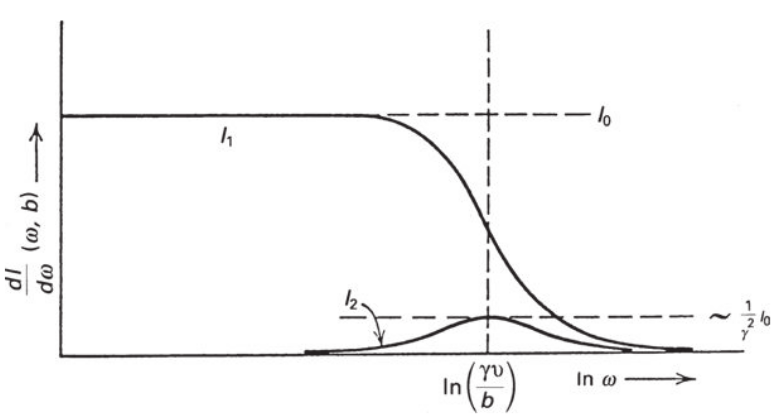
\includegraphics[totalheight=5cm]{plot/brem_jackson}
\caption{The bremsstrahlung spectrum from the acceleration of the electron parallel and perpendicular
to its initial direction of motion as was displayed in \citet{jackson}, or \citet{rybicki:1}.}
\label{jackson_brem} 
\end{figure}

Now we can integrate over all the collision parameters which contribute to the radiation at frequency 
$\omega$: 
\begin{equation}
 \label{brems_final}
I(\omega') = \int_{b'_{min}}^{b'_{max}} 2 \pi b' \gamma N \upsilon K \mathrm{d}b' = \frac{Z^6 e^6 \gamma N}{12\pi^3 \varepsilon_0^3 c^3 m_e^2} \frac{1}{\upsilon} \mathrm{ln}\left ( \frac{b'_{max}}{b'_{min}} \right ),
\end{equation}
note that if the electron is moving by relativistic speed, because of the relativistic length contractions,
it observed more nuclei enhanced by a factor $\gamma$. $N' = \gamma N$, where $N$ is nuclear density .   

\subsection{Thermal bremsstrahlung}
In previous sub-section we derive the breaking radiation spectrum for one electron, but in real plasma 
at temperature T is necessary to integrate single partition spectrum over the collision parameters 
and over the Maxwell distribution of electron velocities 
\begin{equation}
\label{them_brems}
N_e(\upsilon)\mathrm{d}\upsilon = 4 \pi N_e \left ( \frac{m_e}{2 \pi k T} \right )^{2/3}\upsilon^2 \mathrm{exp}\left ( -\frac{m_e \upsilon^2}{2kT} \right ) \mathrm{d}\upsilon . 
\end{equation}
The approximate expression for the spectral emissivity of a plasma of electron density $N_e$ in the low 
frequency limit is 
\begin{equation}
 \label{low_f_tbrem}
I(\omega)\approx \frac{Z^2e^6NN_e}{12\sqrt{3}\pi^3\varepsilon_0^3c^3m_e^2}\left ( \frac{m_e}{kT} \right )^{1/2} \: g(\omega,T),
\end{equation}
where $g(\omega , T)$ is known as Gaunt factor.
It is important to realize that the low frequency thermal bremsstrahlung spectrum is almost independent of 
frequency, the only dependence upon $\omega$ comes from the slightly varying function in the Gaunt factor. 

At the high frequencies the spectrum of thermal bremsstrahlung exponentially cuts off according to 
$\mathrm{exp}(-\hbar \omega / kT)$. This behavior is reflecting the exponential decrease in the 
electrons population in hard energy tail of Maxwell distribution. 

Finally, we can get the total energy loss by the plasma by integrating the spectral emissivity over 
all possible frequencies, because of the exponential cut-off, the integration should be helds from $0$ to 
$\omega = kT/ \hbar$ which leads to 
\begin{equation}
 \label{brem4}
-\frac{\mathrm{d}E}{\mathrm{d}t} = \mathrm{(constant)} \: Z^2T^{1/2}\bar{g}N N_e .
\end{equation}

Detailed calculations give the following results, int terms of frequency $\upsilon$ rather then the angular
frequency $\omega$. The spectral plasma emissivity according to \citet{longair:1} is
\begin{equation}
 \label{tbremss1}
\begin{split}
 K_\upsilon &= \frac{1}{3\pi^2}\left ( \frac{\pi}{6} \right )^{1/2} \frac{Z^2e^6}{\varepsilon^3_0c^3m_e^2} \left ( \frac{m_e}{kT} \right )^{1/2} \: g(\upsilon,T) N N_e \mathrm{exp}\left ( -\frac{h \upsilon}{kT} \right ), \\
 & = 6.8 \times 10^{-51} Z^2 T^{-1/2} N N_e g(\upsilon, T) \mathrm{exp}\left ( - \frac{h \upsilon}{kT} \right ) \mathrm{W\,m^{-3}\,Hz^{-1}},     
\end{split}
\end{equation}
where both: densities of electrons $N_e$ and of nuclei $N$ are in barticles per $\mathrm{m^3}$. At frequencies 
$h \upsilon \ll kT$, the Gaunt factor has only a logarithmic dependence on the frequency.  
Therefore for radio and X-ray wavelengths are suitable following forms:
\begin{equation}
 \label{approx_brem}
\begin{split}
 \mathrm{Radio:} & \: \:g(\upsilon, T) = \frac{\sqrt{3}}{2\pi}\left [ \mathrm{ln} \left ( \frac{128\varepsilon_0^2k^3T^3}{m_e e^4 \upsilon^2 Z^2} \right ) - \gamma^{1/2} \right ] ,\\
 \mathrm{X-ray:} & \: \:g(\upsilon, T) = \frac{\sqrt{3}}{2\pi} \mathrm{ln} \left ( \frac{kT}{h\upsilon} \right ),
\end{split}
\end{equation}
where $\gamma = 0.577$ is the Euler's constant. 

The total loss rate of the plasma is
\begin{equation}
 \label{thermbrems_f}
-\left ( \frac{\mathrm{d}E}{\mathrm{d}t} \right )_{brems} = 1.435 \times10^{-40}Z^2T^{1/2}\bar{g}N N_e \: \mathrm{W\:m^{-3}}.
\end{equation}
Detailed calculation show that the average value of the Gaunt factor $\bar{g}$ lies in the range 
$1.1 - 1.5$, then $\bar{g} = 1.2$ will be a good approximation (\citet{longair:1}).  
To apply a suitable Gaunt factors in the thermal bremsstrahlung formula is nontrivial and complex task.
Several useful papers about suitable Gaunt factors were published. One of the more recent is that from 
\citet{1998MNRAS.300..321S}.

\section{PSR model}

By using previous results and assumptions, we can now find an explicit column solution. We specified 
that the cooling process in PSR is thermal bremsstrahlung and also that other mechanisms such Compton 
and cyclotron cooling are negligible in IPs case. We know that the electron and ion temperature will 
remain very stable. We also expect, that shock height (see fig. \ref{psr1} where $z_0 – R_{wd} = D$ 
is shock distance from WD surface) is $D < R_{wd}$, therefore we can adopt one dimensional geometry 
with vertical coordinate $z$ as is showed on the fig. \ref{psr1}.

The structure of the stationary PSR in plane--parallel one--dimensional geometry is described
(see e.g. \citet{2005A&A...435..191S}, \citet{1999MNRAS.306..684C} or \citet{accpower:1}) by the
mass continuity equation:
\begin{equation}
 \label{mas_con}
\frac{\mathrm{d}}{\mathrm{d}z}(\rho \upsilon) = 0   \:,
\end{equation}
the momentum equation
\begin{equation}
 \label{momentum_eq}
\frac{\mathrm{d}}{\mathrm{d}z}(\rho \upsilon^2 + P) = -\frac{GM_{wd}}{z^2}\rho             \:,
\end{equation}
the energy equation 
\begin{equation}
 \label{ener_eq}
\upsilon \frac{\mathrm{d}P}{\mathrm{d}z} + \gamma P \frac{\mathrm{d}\upsilon}{\mathrm{d}z} = -(\gamma -1)\Lambda    \:,
\end{equation}
and also by the ideal gas law:
\begin{equation}
 \label{ideal_gas_l}
P = \frac{\rho k T}{\mu m_H}   \:.
\end{equation}
where $z$ is a spatial coordninate (see fig.\ref{psr1}), $\upsilon$ is the gas velocity, $\rho$ is the gas 
density, $T$ is the temperature, $P$ is the gas pressure, $\mu=0.62$ is the mean molecular weight of the fully
ionized solar composition matter and $\gamma = 5/3$ is the adiabatic index. $\Lambda$ is the cooling rate:
\begin{equation}
 \label{cool_rate_L}
\Lambda = \left( \frac{\rho}{\mu m_H}\right)^2 \Lambda_N(T),
\end{equation}
where the cooling function $\Lambda_N(T)$ for low densities plasma with $\mu=0.62$ is 
tabulated by \citet{1993ApJS...88..253S}.

The Eq.\eqref{mas_con} can be interested with result:
\begin{equation}
 \label{res_int_mas_con}
\rho \upsilon = a,
\end{equation}
where tha $a$ is local mass accretion rate of dimension $\mathrm{g\:cm^{-2}\:s^{-1}}$
This is the free parameter of the model, but according to \citet{2005A&A...435..191S} the spectrum of 
emergent radiation in PSR is rather insensitive to this parameter with reasonable limits.     

By using the substitution $z' = z_0 - z$ where $z_0$ is the shock--wave coordinate (see fig. \ref{psr1}),
and with $g(z') = (GM_{wd})/(z_0 - z')^2$ we should rewrite the Eq.\eqref{momentum_eq} and Eq.\eqref{ener_eq} 
with knowledge of Eq.\eqref{res_int_mas_con}:
\begin{equation}
 \label{big_ass_eq1}
\frac{\mathrm{d} \upsilon}{\mathrm{d} z'} = g(z')\frac{1}{\upsilon}-\frac{1}{a}\frac{\mathrm{d}P}{\mathrm{d}z'} \:,
\end{equation}
\begin{equation}
 \label{big_ass_eq2}
\frac{\mathrm{d}P}{\mathrm{d}z'} = \frac{(\gamma -1) \Lambda a + g(z')\gamma Pa / \upsilon}{\gamma P -a / \upsilon } \:.
\end{equation}

The equations \eqref{big_ass_eq1} and \eqref{big_ass_eq2} could be solved by using sufficient 
numerical method, e.g \citet{2005A&A...435..191S} and  \citet{1999MNRAS.306..684C} used shooting 
method from $z=z_0(z'=0)$ to $z = R_{wd}(z'=z_0-R_{wd})$ with boundary condition at $z=z_0$ with results:
\begin{equation}
 \label{res_shoot}
\begin{split}
\upsilon_0 &= 0.25\sqrt{2GM_{wd}/z_0}\:,\\
\rho_0 &= a / \upsilon_0\:,\\
P_0 &= 3a\upsilon_0\:,\\
T_0 &= 3\frac{\mu m_H}{k}\upsilon_0^2\:. 
\end{split}
\end{equation}
The equation which ties up the $R_{wd}$ and $M_{wd}$ is typically used that one from 
the \citet{1972ApJ...175..417N} article:
\begin{equation}
 \label{rwd_mwd}
R_{wd} = 7.8 \times 10^8 \left[ \left( \frac{1.44\mathrm{M_\odot}}{M_{wd}} \right)^{2/3} -\left( \frac{M_{wd}}{1.44\mathrm{M_\odot}} \right)^{2/3} \right]^{1/2}\:\mathrm{cm}\:.
\end{equation}

The simple analytical model from the \citet{accpower:1}, based on assumption of the constant pressure 
in the PSR region can by also used as follows:
\begin{equation}
 \label{king_ana}
\begin{split}
T(z) &= T_0 \left( \frac{z - R_{wd}}{z_0 - R_{wd}}\right)^{2/5}\:,\\
\rho(z) &= \rho_0 \left( \frac{z - R_{wd}}{z_0 - R_{wd}}\right)^{-2/5}\:.
\end{split}
\end{equation}

\begin{figure}[hbt]
\centering
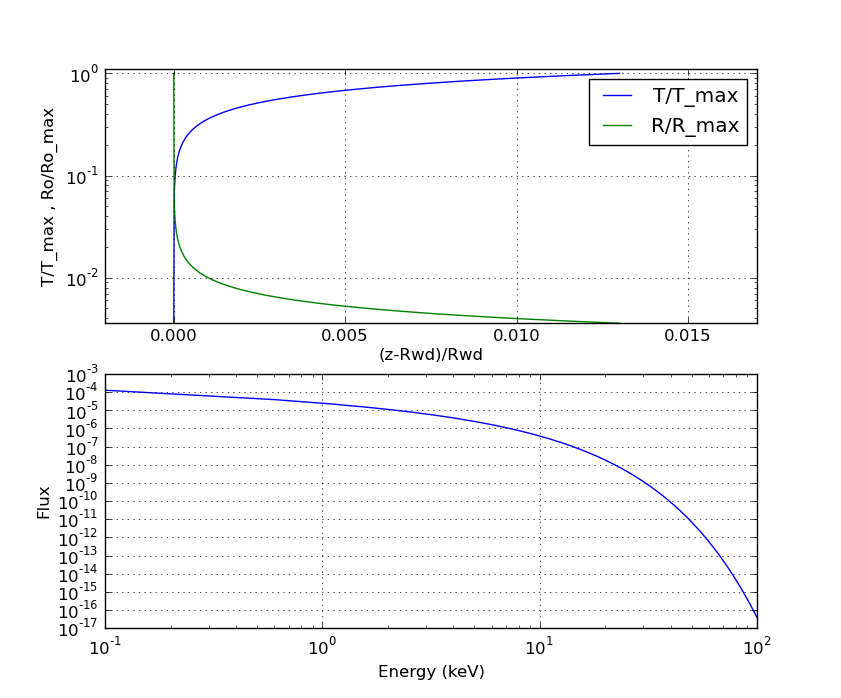
\includegraphics[totalheight=10cm]{model/image}
\caption{\textit{Top:} the temperature and density profiles for the analytical model from \citet{accpower:1}. The input 
parameters for script was: $M_{wd} = 0.7\mathrm{M_\odot}$ and shock distance from WD 
surface $0.013 R_{wd}$, $a = 1.0 \mathrm{cm^{-2}\:s^{-1}}$, The coresponding WD radius is $\sim$ 7797km, while the 
resulting $kT_{max} = 29.71\mathrm{\:keV}$.
\textit{Bottom:} the emergent model spectru calculated by suming of the local bremsstrahlung spectra.}
\label{koc_mod} 
\end{figure}

The emergent model spectrum will be calculated by summing of the local bremsstrahlung spectra:
\begin{equation}
 \label{int_spec1}
F_E = \int_{R_{wd}}^{z_0}j(z)\mathrm{d}z,
\end{equation}
where the local spectra were taken in form (\citet{zomb}, \citet{2005A&A...435..191S}): 
\begin{equation}
 \label{loc_spec_zom}
j(z) = 9.52\times 10^{-38} \left( \frac{\rho (z)}{\mu m_H}\right)^2 T(z)^{-1/2} \left(\frac{E}{kT(z)} \right)^{-0.4} \mathrm{exp}\left(-\frac{E}{kT(z)} \right) \:.
\end{equation}



\subsection{WD mass estimations methods}
\citet{1973PThPh..49.1184A_aizu} gives the formula relating the gravitation potential of the WD to the mass and radius:
\begin{equation}
 \label{aizu1}
kT_s = 16 \times \left( \frac{M}{0.5\mathrm{M_{\odot}}}\right)\left( \frac{R}{10^9 \mathrm{cm}}\right)^{-1} \mathrm{keV},
\end{equation}
which can be combined with the Eq.\eqref{rwd_mwd} from the work of \citet{1972ApJ...175..417N}, allowing
us to calculate the mass of the WD from the PSR temperature:   
\begin{equation}
 \label{MWD:1}
\frac{M_{wd}}{\mathrm{M_{\odot}}} = 1.44\times \left[\frac{1}{2} \left( 1+ \sqrt{1+4\times\left(\frac{59}{kT_s}\right)^2} \right) \right]^{-3/4}.
\end{equation}



\chapter{Data reduction and analysis}
In this chapter we describe the results and data analyze threads for both XMM--Newton and INTEGRAL data. 
All data, software and online utilities necessary to finding the data, download and analyze are free 
and runs under \textit{Linux}.  

\section{INTEGRAL}
INTErnational Gamma-Ray Astrophysics Laboratory (INTEGRAL) is the European Space Agency's satellite, 
launched in 2002 from Baikonur Cosmodrome on-board Proton-K launcher. INTEGRAL lies on orbit with 
period 72 hours where the large fraction of its orbit is behind radiation belts. The INTEGRAL service 
module is clone of the XMM-Newton one which significantly reduced construction costs. 
INTEGRAL has four scientific instruments on-board, the IBIS/ISGRI is used in this work. 
\begin{itemize}
 \item \textbf{IBIS} (Imager on-Board the INTEGRAL Satellite) observes in broad band $15\:\mathrm{keV} -
10\:\mathrm{MeV}$.
\item \textbf{SPI} (SPectrometer for INTEGRAL) observes in $20\:\mathrm{keV}-8\:\mathrm{MeV}$, part of the SPI is
also ACS (AntiCoincidence Shield).
\item \textbf{JEM-X} observed in $3 - 35\:\mathrm{keV}$.
\item \textbf{OMC} is an optical monitor sensitive in $500-580\:\mathrm{nm}$.
\end{itemize}

\begin{figure}[!hbt]
\centering
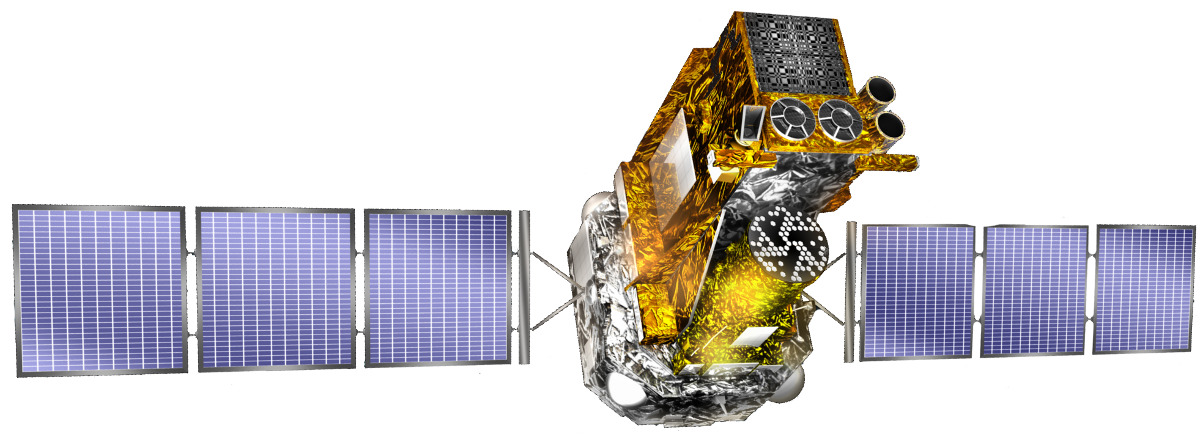
\includegraphics[totalheight=4cm]{integral}
\caption{ESA/INTEGRAL spacecraft with four scientific instrument and 4 ton launch mass is one of the largest European satellites. }
\label{integral1} 
\end{figure}

\subsection{IBIS/ISGRI}
IBIS is a coded mask gamma ray telescope operating in very broad energy range, from the hard X-rays to 
gamma-rays, however its sensitivity strongly decreases with the increasing energy bands. It is an 
imaging detector which uses coded mask. The mask itself its a special coded pattern, that chosen for 
the IBIS detector is based of a cyclic replication of MURA (Modified Uniform Redundant Array) of order 
53, this detection technology is describes in \citet{mask1}.

\begin{table}[hbt!]\footnotesize
\begin{center}
\caption{Scientific parameters of the IBIS instrument on-board INTEGRAL space mission, \citet{osam}.}
\begin{tabular}{|l|l|}
\hline
Operating energy range     & 15 keV -- 10 MeV\\
\hline
Energy resolution (FWHM)   & 7\% at 100 keV\\
                           & 9\% at 1MeV  \\
\hline
Effective area             & ISGRI: 960 $\mathrm{cm^2}$ at 50 keV \\
                           & PICsIT: 870 $\mathrm{cm^2}$ at 300 keV (single events)\\
                           & PICsIT: 275 $\mathrm{cm^2}$ at 1 MeV (multiple events)\\
\hline
FOW                        &$8.3\,^{\circ} \times 8.0\,^{\circ}$ (fully coded) \\
                           &$19\,^{\circ} \times 19\,^{\circ}$ (partially coded, 50\%)\\
\hline
Angular resolution (FWHM)  & 12' \\
\hline
Point source location accuracy & $30''$ at 100 keV \\
$90\%$ error radius      & $<5'$ at 1 MeV \\
\hline
Continum sensitivity, & $3.8 \times 10^{-7}$ at 100 keV \\
photons $\mathrm{cm^{-2}\: s^{-1}\: keV^{-1}}$ & $1 - 2 \times 10^{-7}$ at 1 MeV \\
($3 \sigma$ detection, $\Delta E = E/2$, $10^6$ s integration) &  \\
\hline
Narrow line sensitivity, & $1.3 \times 10^{-5}$ at 100 keV \\
photons $\mathrm{cm^{-2}\: s^{-1}}$ & $4 \times 10^{-5}$ at 1 MeV \\
($3\sigma,\:10^6$ s integration)&  \\
\hline
Absolute timing accuracy $(3 \sigma)$& ISGRI: $61 \:\mathrm{\mu s}$\\
 & PICsIT: 0.976 -- 500 ms (selected from the ground)\\
\hline
\end{tabular}
\end{center}
\end{table}

The IBIS is two layers detector, where the first layer is called ISGRI and second PICsIT. ISGRI is based 
on the cadmium telluride (CdTe), which is semiconductor operating at normal temperatures. The detector 
layer is made of 8 MDUs /footnote{Modular Detector Unit} each having $32\times64$ pixels. The lower 
detector, PICsIT is based on cesium iodide (CsI) crystals. 

The coded mask produced a shadowgram, the photon from the image are distributed across the entire detector, 
but cross-correlation techniques are used for taking a full reconstructed image in fully coded FOV. 
For reconstruct the image in partially coded FOV is necessary to use special cleaning techniques.

\subsection{Data reduction}
For the IBIS/ISGRI data reduction we used the 64-bit version of the Off-line Science Analysis (OSA 9.0) 
software which can be downloaded from INTEGRAL Science Data Center web-pages\footnote{http://www.isdc.unige.ch/integral/}. 
It is necessary to download also the instrument calibration and response data and the latest 
objects reference catalogue.
For suitable data analysis in high energy astrophysics is necessary to use also several 
typical software packages as: ds9, fv, FTOOLS\footnote{See http://heasarc.nasa.gov/lheasoft/}.       
For the reduction itself we used following set of commands in the sequence:

\begin{enumerate}
 \item \verb rbnrmf  was used for creating a rebinning responce matrix for 10 spectral bins in 20--100 keV
 \item \verb og_create  was used for creating observation groups
 \item \verb ibis_science_analysis  package was used for image reconstruction and creating mosaics
 \item \verb mosaic_spec  was used for the spectral extraction from the final mosaics
\end{enumerate}


\section{XMM-Newton}
The European Space Agency's (ESA) X-ray Multi-Mirror Mission (XMM-Newton) was launched by an Ariane 504 
on December 10th 1999. The XMM weighs 3.8 tons and caries three X-ray telescopes each contains 58 Wolter I 
grazing -- incidence mirrors. The instruments on-board are three European Photon Imaging Cameras (EPIC) 
and two Reflection Grating Spectrometers (RGS).

\begin{figure}[!hbt]
\centering
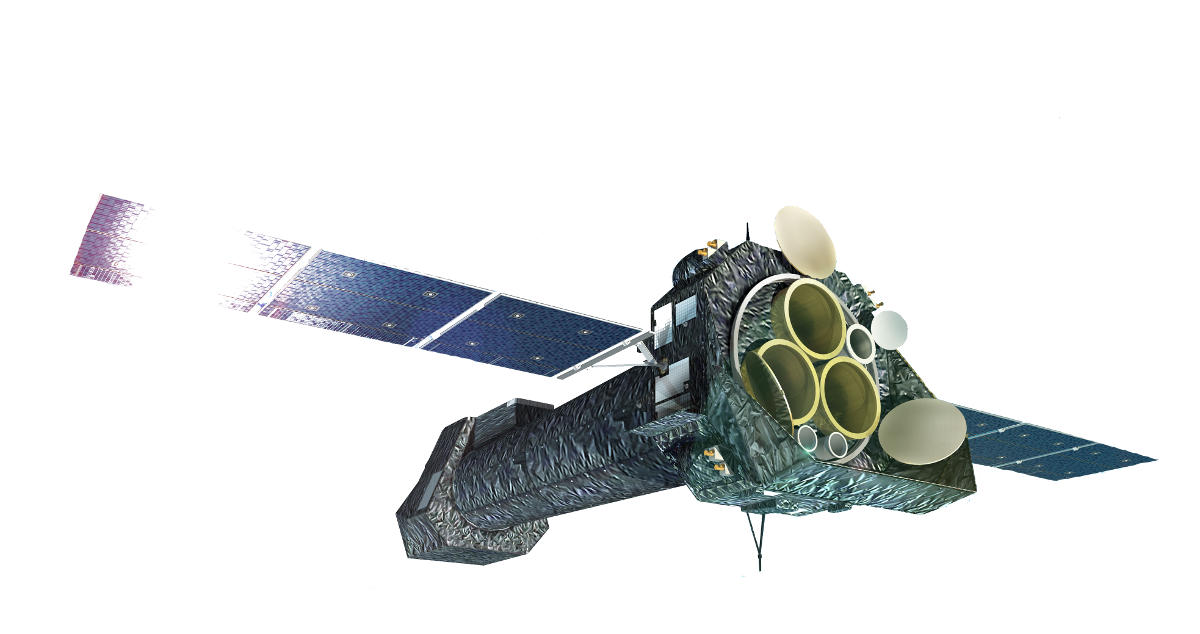
\includegraphics[totalheight=6cm]{XMM}
\caption{The XMM-Newton (X-ray Multi-Mirror Mission) is one off the most successful space mission of all time.}
\label{xmmn1} 
\end{figure}

Two of the cameras are Metal Oxide Semi-conductor (MOS) CCD arrays. Third camera is pn CCD camera. 
There is also an optical telescope on-board, the 30 cm diameter Ritchey---Chretien observing in the
UV/optical band.  

In each MOS there area seven EEV type 22 front illuminated CCDs. The six surrounding CCDs are 
stepped towards because of the focal plane curvature while the middle one is at the focal point of 
the X-ray telescope. The MOS cameras are sensitive in the energy range 0.2 to 10 keV.All the EPIC CCDs 
operate in photon counting mode. In the case of MOS cameras, the central CCD can be operated separately. 

\begin{figure}[!hbt]
\centering
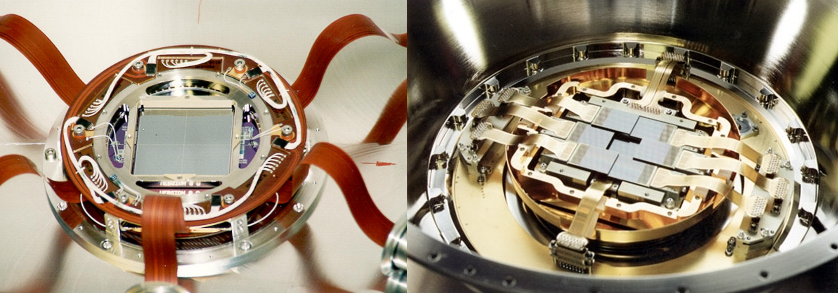
\includegraphics[totalheight=4cm]{plot/epic}
\caption{EPIC -- European Photon Imaging Camera consists of \textit{(left image)} pn ccd and 
\textit{(right image)} two MOS CCDs.}
\label{xmmn1_epic} 
\end{figure}


\subsection{Data reduction}
For the data acquisition was used XMM-Newton Science Archive (XSA)\footnote{http://xmm.esac.esa.int/xsa/} and
candidates was selected from the Koji Mukai online catalog of IPs and IP candidates\footnote{http://asd.gsfc.nasa.gov/Koji.Mukai/iphome/catalog/alpha.html}.
From the catalogue of 92 IPs/IP candidates and 33 others systems was selected only strongly confirmed 
(in catalogue marked as $^{\bigstar \bigstar \bigstar \bigstar \bigstar}$) 
and confirmed (marked as $^{\bigstar \bigstar \bigstar \bigstar}$) systems. 

This leads to selection of 25 sources:

\begin{footnotesize} 
\begin{tabular}{l l l }\footnotesize
1RXS J005528.0+461143 & 1RXS J070407.9+262501 & 1RXS J180340.0+401214 \\
AO Psc & BY Cam & EI UMa \\
EX Hya & FO Aqr & GK Per\\
HT Cam & IGR J00234+6141 & IGR J15094-6649 \\
IGR J17195-4100 & IGR J17303-0601 & IGR J21335+5105\\
MU Cam & NY Lup& PQ Gem\\
SDSS J233325 & UU Col& V1223 Sgr\\
V2069 Cyg & V2400 Oph &V405 Aur \\
XY Ari & &  \\
\end{tabular}
\end{footnotesize}

For all the public available pointings for all the 25 sources the following data reduction procedures 
took place. The XMM-Newton Science Analysis System (SAS) version 11.0.0 for Feora 32-bit Linux 
was used and executed by simple bash skript: 
\begin{tiny}
\begin{verbatim}
#!/bin/bash
#this script should run simple xmm MOS spectral analysis for future spectral extraction
alias ldir="ls -l | egrep '^d'"
alias xmm32='. /home/mkocka/diplomka/soft/sas32/xmmsas_20110223_1801/setsas.sh'
export HEADAS=/home/mkocka/diplomka/soft/heasoft-6.11/x86_64-unknown-linux-gnu-libc2.14
export SAS_CCFPATH=/home/mkocka/diplomka/soft/sas/xmmsas_20110223_1801/ccf
alias heainit=". $HEADAS/headas-init.sh"
cd /home/mkocka/diplomka/work/xmm1
export LDR=`pwd`
heainit
xmm32
cd $SAS_DIR
export LD_LIBRARY_PATH=$LD_LIBRARY_PATH:`pwd`/libextra
export PATH=$PATH:/home/koci/XMM/xmmsas_20100423_1801/bin
cd $LDR
for i in * 
        do cd $i 
        for j in `ldir | awk '{print $9}'`
                do cd $j/odf
                export SAS_ODF=`pwd`
                if [ -f *.SAS ]; then rm *.SAS; fi
                cifbuild	
                export SAS_CCF=`pwd`/ccf.cif 
                odfingest
                cd ..
                mkdir MOS
                cd MOS
                emchain
                mos-filter 
                for k in `ls *clean*` 
                        do evselect table=$k imagebinning=binSize imageset=image_$k \
                        withimageset=yes xcolumn=X ycolumn=Y ximagebinsize=64 yimagebinsize=64
                        done 
                        cd ../..
        done
        cd ..
done 
\end{verbatim}
\end{tiny}

In the next step of the analysis thread was checked which of the 25 IPs observed by XMM has been also 
observed by INTEGRAL and have enough exposures for necessary spectral extraction. The seven sources 
was been selected for spectral extraction.   

The spectra from all suitable MOS observations was taken by standard SAS data product extraction. The 
following commands took place:
\begin{enumerate}
 \item \verb evselect   was used for extraction of the source and background spectrum.
 \item \verb rmfgen   was used for creating a redistribution matrix for the previously extracted spectrum.
 \item \verb arfgen  was used for genarate an ancillary file.
 \item \verb specgroup  was used for rebinig  the spectrum and link associated files.
\end{enumerate}

\section{Spectral analysis and results}
The spectra for the selected seven IPs from XMM-Newton/MOS and INTEGRAL/ISGRI were analyzed by the X-ray 
spectral fitting package Xspec 12.7.0 \citet{1996ASPC..101...17A}. Xspec is a part of the NASA HEASOFT 
6.0 software dedicated mostly for the data reduction and analysis of the data the from various high energy space 
missions.

Xspec is a powerful tool enabling fitting the high energy spectra by various models. That is exactly 
what was necessary for the PSR temperature determination. Because of a poor quality of the INTEGRAL/IBIS 
data, we decided to fit the simple combined model \verb wabs(bremss+bb+ga) and \verb wabs(bremss) for the
ISGRI data only.   

\subsection{Xspec models}
The spectra were fitted by the combined model. In the joint MOS and ISGRI spectral fitting, three additive and one
multiplicative model was used. 
The \textbf{wabs} multiplicative module is a photo-electric absorption
\begin{equation}
\label{wabs}
 M(E)= \mathrm{exp}\left[ -n_H \sigma (E)\right]\:,
\end{equation}
where $s(E)$ is the photo-electric cross-section, $n_H$ is the equivalent hydrogen column.
The \textbf{bremss} is a thermal bremsstrahlung spectrum with one parameter, which is the plasma
temperature $T_s$ in keV.
\begin{equation}
 \label{brems}
\frac{3.02\times10^{-15}}{4\pi D} \int n_e n_I \mathrm{d}V\:,
\end{equation}
where $D$ is the distance to the source in cm nad $n_e$, $n_I$ are the electron and ion densities.    
The \textbf{bb} is the black body spectrum:
\begin{equation}
 \label{bb}
A(E) = \frac{K\times8.0525E^2 \mathrm{d} E }{(kT)^4 [\mathrm{exp}(E/kT)-1 ]}\:.
\end{equation}
The \textbf{ga} is a simple gaussian line profile. If the width is $\leq 0$, then it is treated as the 
delta function. The gaussian was used for elimination of iron 6.4 keV lines, as can be seen in all MOS spectra e.g. Fig.\ref{sp4}. 
\begin{equation}
 \label{gaus}
A(E) = K \frac{1}{\sigma \sqrt{2\pi}}\: \mathrm{exp}\left( \frac{-(E-E_x)^2}{2\sigma^2} \right)\:.
\end{equation}
 
\section{Results}
Data for the 25 IPs from the XMM-Newton science archive was downloaded and pre-analyzed. After the cross-correlation with INTEGRAL/IBIS observations, the 7 IPs 
were selected for the closer analysis. The EPIC/MOS and INTEGRAL/ISGRI spectra were created by the dedicated software: OSA 9.0 for the IBIS/ISGRI data 
processing and XMM/SAS 11.0.0 for EPIC cameras.

The nine spectra were analyzed using Xspec software package. There were two spectra obtained solely from INTEGRAL/IBIS: for NY Lup and IGR J21335+5105, and seven 
spectra for the selected IPs from the both detectors. The results of the spectral preparation are in Table \ref{RES1} and the results from Xspec 
spectral fitting are in the Table \ref{RES2}. The spectra figures follows.   

The WDs masses were determined using $T_s$ results from the fitting in Table \ref{RES2} together with the Eq.\eqref{MWD:1}

\section{Discussion}
The methods described in Chap. 4 are the best way to determine the WDs masses in the binary systems with 
column accretion by the other means than the optical spectroscopy. However, the observations in X-rays bands are very 
finicky. While the soft X-rays data obtained by XMM-Newton are of a very good quality, the hard X-rays 
data are not. The INTEGRAL/ISGRI is a very sensitive space telescope, but the long time exposures needed 
for good spectra of faint objects are very hard to reduce. The main problem is the calibration, mostly 
because of the radiation self response of the detector. This could be the reason why the over 1Msec ISGRI 
exposures in this work provide spectra of a such poor quality. 

On the other hand, even with poor quality spectra and several threats in the processing, these 
simple methods were able to determine the WD masses with a reasonable precision in the comparison with the previous
 observations, as we can see in the result table \ref{RES2} and in the comparison table \ref{pmass}.


\begin{sidewaystable}
\begin{center}
\caption{Summary of the observations. Columns give the object name, coordinates of the source, its orbital period and distance, XMM-Newton 
observation ID, total exposures times for MOS1 and MOS2, total exposures for IBIS/ISGRI, and period of INTEGRAL observations, 
the IPs are ordering according to their RA.}
\begin{tabular}{lrrlllllrr}
\hline
\hline
     &                         &                          &$\mathrm{P_{orb}}$ & Dist &XMM      & \multicolumn{2}{c}{Exp. time [ks]}&Exp. time [ks] & Last obs.  \\
obj. & Ra $\mathrm{[^{\circ}]}$& Dec $\mathrm{[^{\circ}]}$&(min)            &(pc)  &obs. ID  & MOS1&MOS2                         & IBIS/ISGRI    & IBIS/ISGRI \\ 
\hline
IGR J15094-6649&  227.358  & -66.823 &353.4&--& 0551430301&31.61     & 31.62& 592.46      &    2008-07-24                 \\
NY Lup         &  237.060  & -45.479 &574.2&540-840& 0105460301&21.40     & 21.40& 1589.29     &    2005-04-08                \\
V2400 Oph      &  258.152  & -24.245 &205.8&300& 0105460101&10.07     &10.12& 1368.89     &      2009-03-07                \\
IGR J17195-4100&  259.899  & -41.014 &240.3&110& 0601270201&33.62     &33.62&  878.12    &     2008-10-23              \\
IGR J17303-0601&  262.589  &  -5.992 &924&--& 0302100201&13.28     &13.28&   248.62   &       2008-04-21              \\
V1223 Sgr      &  283.759  & -31.163 &201.9&527& 0145050101&38.66     &38.67&   264.66  &     2006-11-09               \\
IGR J21335+5105&  323.375  &  51.092 &431.6&1400& 0302100101&16.59     &16.40 & 1589.68    &  2009-05-22                   \\
\hline
\end{tabular}
\label{RES1}
\end{center}
\end{sidewaystable}


\begin{sidewaystable}
\begin{center}
\caption{Summary of the spectral analysis. For the each IP the same spectral model was used fitted in by Xspec (X-ray spectral fitting package). Columns gives the IP name, used model, determined shock temperature, calculated mass, and fluxes from model in MOS and ISGRI bands. The last column is chi-squared from the fit.}
\begin{tabular}{lcrrrrrr}
\hline
\hline
     & Xspec & $\mathrm{kT_s}$& $\mathrm{M_{wd}}$   & Flux 1--10 keV                      & Flux 20--100 keV                      &         \\
obj. & model & (keV)          & $\mathrm{M_{\odot}}$& $\mathrm{photons\:cm^{-2}\:s^{-1}}$ & $\mathrm{photons\:cm^{-2}\:s^{-1}}$& $\mathrm{\chi}^2$         \\ 
\hline
IGR J15094-6649    & wabs(bremss+bb+ga) & 18.7 $\pm$ 53  & 0.40  $\pm$ 0.83  &0.0022639&0.0018200&1.297 \\
NY Lup             & wabs(bremss+bb+ga) & 150 $\pm$ 200  & 1.26 $\pm$ 1.33 &0.0042067 &0.0012044&4.036      \\
NY Lup $^b$	   & wabs*bremss        & 53.7 $\pm$ 15.5 &  0.84  $\pm$ 0.33  & ---&0.0013193 & 1.7\\
V2400 Oph          & wabs(bremss+bb+ga) & 31.3 $\pm$ 16.0      &0.59 $\pm$ 0.34&0.0057836&0.0021225&      1.122      \\
IGR J17195-4100    & wabs(bremss+bb+ga) & 13.6 $\pm$ 4.4       & 0.30 $\pm$ 0.11&0.0053613&0.0001013& 1.297 \\
IGR J17303-0601    & wabs(bremss+bb+ga) & 68.7 $\pm$ 74.5     & 0.97 $\pm$ 1.0 &0.0026358& ---$^a$&  0.754        \\
V1223 Sgr          & wabs(bremss+bb+ga) & 41.1 $\pm$ 37.7      &0.71 $\pm$ 0.67&0.0031016&0.0018271&  1.959           \\
IGR J21335+5105    & wabs(bremss+bb+ga) & 40.6 $\pm$ 32.3      &0.71$\pm$ 0.60&0.0031016& 0.0018271&        1.297        \\
IGR J21335+5105$^b$& wabs(bremss+ga)    & 54.7 $\pm$ 7.5      &0.85 $\pm$ 0.17 &---& 0.0019385&        2.0        \\
\hline
\footnotesize
$^a$ not calculated& &&&&& \\
\footnotesize
$^b$ only INTEGRAL/ISGRI data \\
\hline
\end{tabular}
\label{RES2}
\end{center}
\end{sidewaystable}

\begin{figure}[!hbt]
\centering
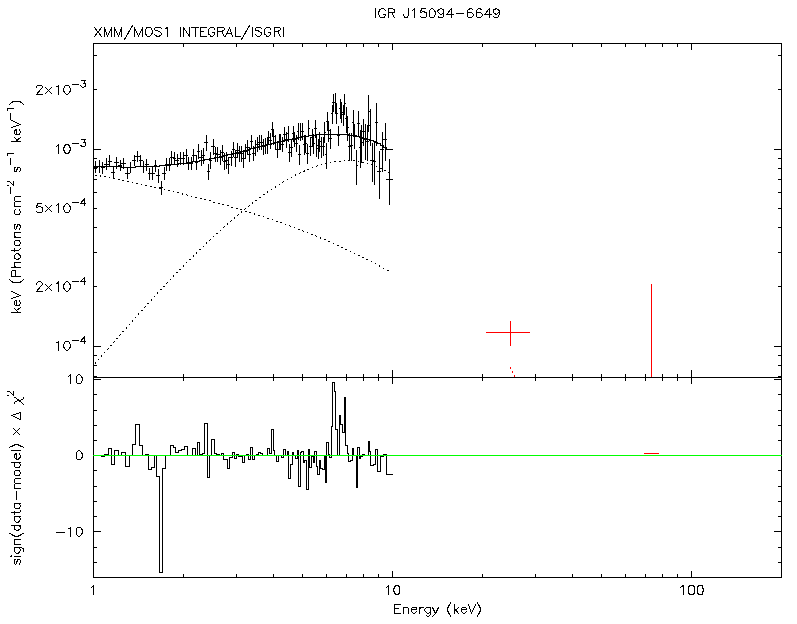
\includegraphics[totalheight=8cm]{spec/1}
\caption{The combined spectrum of IGR J15094-6649 from XMM-Newton EPIC/MOS1 camera and INTEGRAL/ISGRI, unfortunately the INTEGRAL data have a poor quality due to the high X-ray background counts. 
The results of the fit: $T_s = 18.7 \pm 53\:\mathrm{K}$ and $M_{wd} = 0.4 \pm 0.83 \:\mathrm{M_{\odot}}$.}
\label{sp1} 
\end{figure}

\begin{figure}[!hbt]
\centering
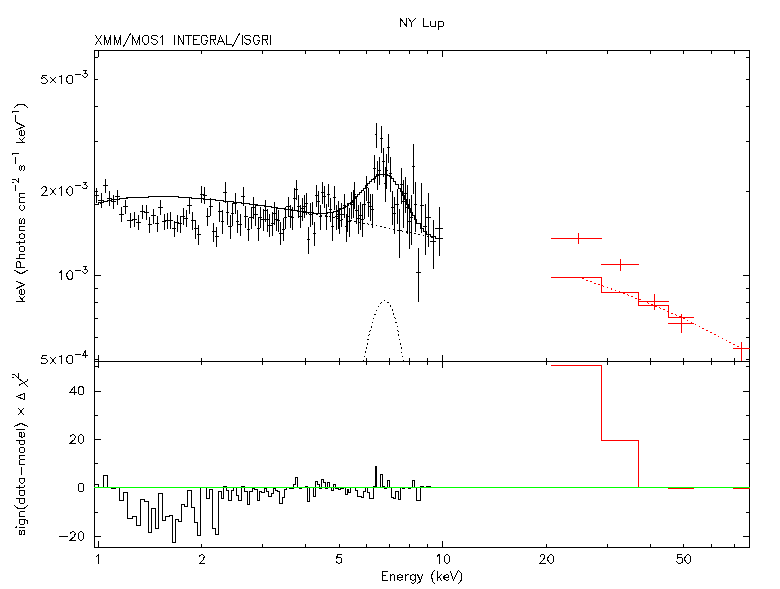
\includegraphics[totalheight=8cm]{spec/2}
\caption{The combined spectrum of NY Lup from EPIC/MOS1 and ISGRI, results of the fit are in table \ref{RES2}.}
\label{sp2} 
\end{figure}

\begin{figure}[!hbt]
\centering
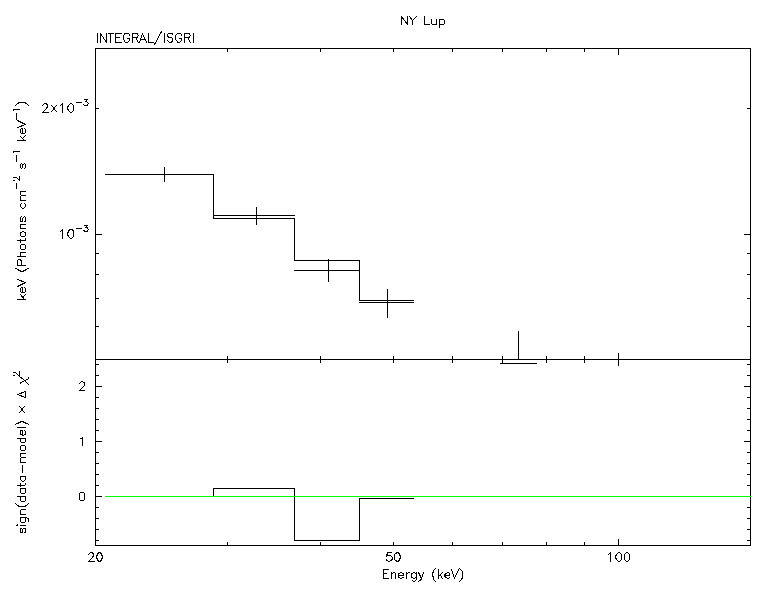
\includegraphics[totalheight=8cm]{spec/2I}
\caption{The ISGRI spectrum of NY Lup, from wabs(bremss) model fit was established: $T_s=53.7 \pm 15.5 \: \mathrm{K}$ and $M_{wd} = 0.84 \pm 0.33 \: \mathrm{M_{\odot}}$ (see table \ref{RES2}).} 
\label{sp2I} 
\end{figure}


\begin{figure}[!hbt]
\centering
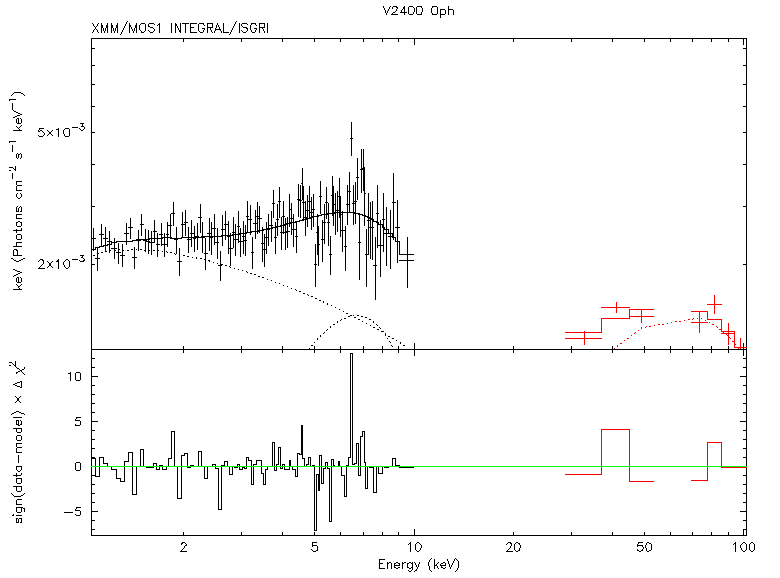
\includegraphics[totalheight=8cm]{spec/3}
\caption{V2400 Oph spectra from EPIC/MOS1 and ISGRI (see table \ref{RES2} for details).}
\label{sp3} 
\end{figure}

\begin{figure}[!hbt]
\centering
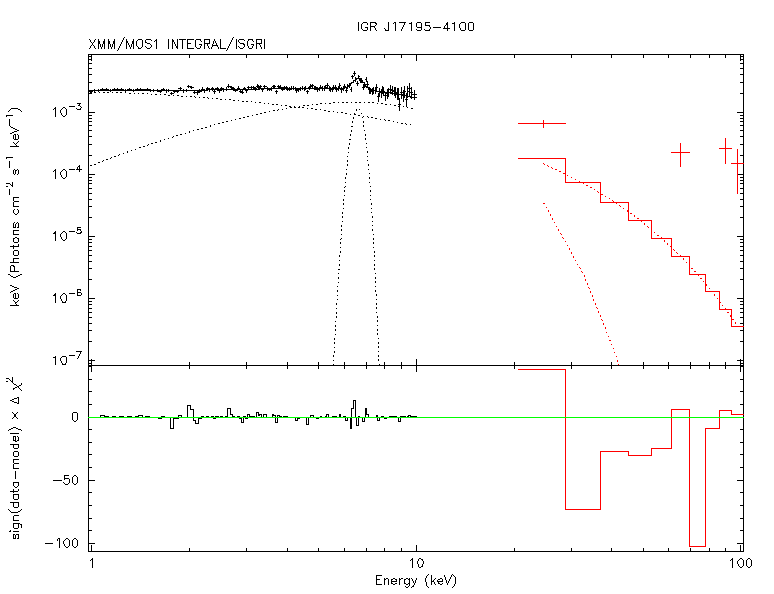
\includegraphics[totalheight=8cm]{spec/4}
\caption{IGR J17195-4100 spectra, unfornately the ISGRI data have a poor quality, for details see table \ref{RES2}. }
\label{sp4} 
\end{figure}

\begin{figure}[!hbt]
\centering
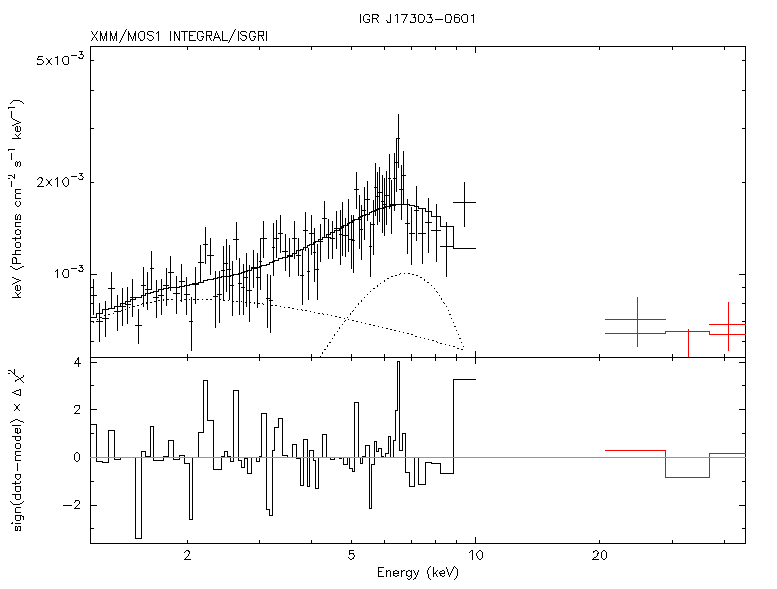
\includegraphics[totalheight=8cm]{spec/5}
\caption{Spectra of IGR J17303-0601, for for details see table \ref{RES2}. }
\label{sp5} 
\end{figure}

\begin{figure}[!hbt]
\centering
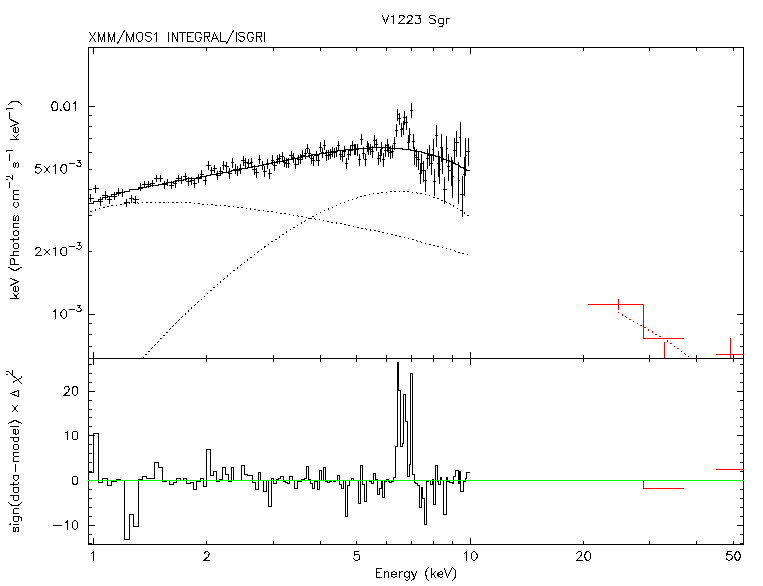
\includegraphics[totalheight=8cm]{spec/6}
\caption{Spectra of V1223 Sgr, for details see table \ref{RES2}. }
\label{sp6} 
\end{figure}


\begin{figure}[!hbt]
\centering
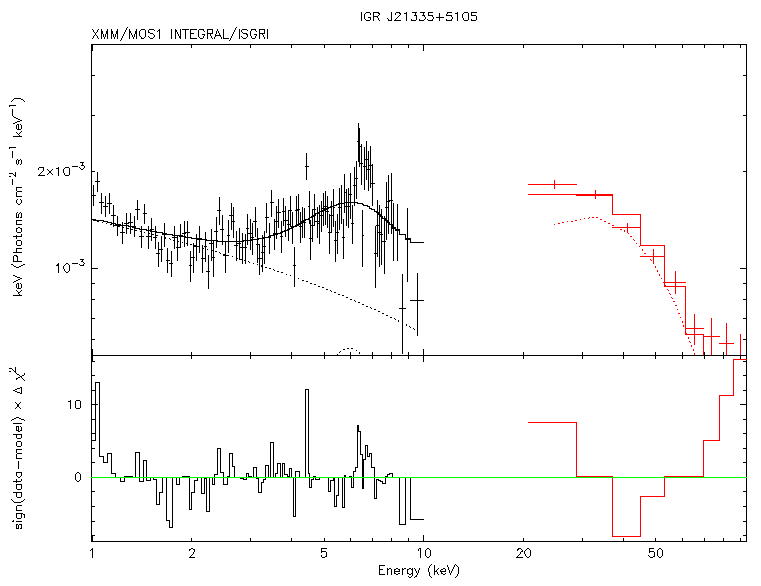
\includegraphics[totalheight=8cm]{spec/7}
\caption{Spectra of IGR J21335+5105, for for details see table \ref{RES2}. }
\label{sp7} 
\end{figure}

\begin{figure}[!hbt]
\centering
\includegraphics[totalheight=8cm]{spec/7I}
\caption{ISGRI spectra of IP IGR J21335+5105, while the combined spectra show a poor quality of the fit, this is the only ISGRI spectrum fited by simple Xspec wabs(bremss+ga) model
showing good results: $T_s = 54.7 \pm 7.5 \mathrm{K}$ and therefore $M_{wd} = 0.85 \pm 0.17 \mathrm{M_{\odot}}$ . }
\label{sp7I} 
\end{figure}

\begin{sidewaystable}
\begin{center}
\caption{Estimations of the WD masses for the 7 IPs studied in this work from previous reports.}
\begin{tabular}{lllllll}
\hline
\hline
%\multicolumn{2}{c}{Item} \\
System & Suzaku$^a$ & Swift$^b$ & RXTE$^c$ & RXTE$^d$ &  ASCA$^e$& This work  \\
       & XIS+HXD & BAT& PCA+HEXTE & PCA &  SIS & XMM \& Integral                     \\
       & $M_{WD}$ &$M_{WD}$ &$M_{WD} $&$M_{WD}$ &$M_{WD}$ &$M_{WD}$ \\
\hline
 NY Lup        & 1.15$^{+0.08}_{-0.07}$  & 1.09 $\pm$ 0.07      &          &     &               &  0.84 $\pm$ 0.17         \\
 V2400 Oph     & 0.62$^{+0.06}_{-0.05}$   &  0.81 $\pm$ 0.10      &  0.59 $\pm$ 0.05       &  0.71$^{+0.07}_{-0.03}$          &  0.68$^{+0.42}_{-0.24}$       &        0.59 $\pm$ 0.34   \\
 V1223 Sgr&     0.75$^{+0.05}_{-0.05}$    &0.65 $\pm$ 0.04        & 0.95 $\pm$ 0.05         & 1.07$^{+0.08}_{-0.09}$          &    1.28($>$0.84)      &         0.71 $\pm$ 0.67  \\
 IGR J17195-4100&  0.38$^{+0.05}_{-0.05}$       &        &          &     &               &     0.30 $\pm$ 0.11      \\
 IGR J21335+5105& 0.91$^{+0.19}_{-0.17}$  &    0.91 $\pm$ 0.06     &          &           &         &      0.71 $\pm$ 0.60     \\
 IGR J15094-6649&         &        &          &     &      &                0.40 $\pm$ 0.83   \\
 IGR J17303-0601&   1.06$^{+0.19}_{-0.14}$   & 1.08 $\pm$ 0.07       &          &     &      &                  0.97 $\pm$ 1.0  \\
\hline
\footnotesize
$^a$ Yuasa et al. (2010) &&&&&&\\
\footnotesize
$^b$ Brunschweiger et al. (2009) &&&&&&\\
\footnotesize
$^c$ Suleimnaov et al. (2004)&&&&&&\\
\footnotesize
$^d$ Ramsay (2000)&&&&&&\\
\footnotesize
$^e$ Ezuka \& Ishida (1999) &&&&&&\\
\hline
\end{tabular}
\label{p_mass}
\end{center}
\end{sidewaystable}

\chapter{Conclusions}
In this thesis we dealt with the various aspects of the accretion processes in magnetic white dwarf 
located in binary systems called cataclysmic variable stars. We were particularly interested in 
intermediate polars. In Chap. 1 we described the main motivations behind this work and we briefly 
summarized the history of observations these objects in the various wavelengths. In Chap. 2 we 
provided a primer on physics of white dwarfs including the concepts of Fermi energy, degeneracy, 
the Chandrasekhar limit. Further on we classify white dwarfs in distinct sub-classes. 

Chap. 3 focuses on cataclysmic variable stars. We briefly discussed various physics processes 
taking places in cataclysmic variables. We are especially focused on magnetic CVs and discussed 
their characteristic X-ray spectra, as we can see on Fig. \ref{kriv_1}.

Chap 4. is an extensive treatise on WD masses in intermediate polars. We also discuss the 
existence of the shock region close to the WD surface and the cooling mechanism in the so 
called post-shock region (PSR). We found out that the radiative cooling of the PSR gas is 
dominated by the bremsstrahlung (free-free) emission. The chapter concludes with a brief 
discussion of several WDs mass estimation methods.

The data acquisition, reduction and analysis is the subject of Chap. 5. Which is the main 
practical part of the thesis. We provide the specification of  instruments on-board 
XMM-Newton and INTEGRAL space missions we used. We used the XMM data from EPIC/MOS 
cameras in 1 – 10 keV and INTEGRAL data from IBIS/ISGRI gamma-ray telescope in 20 – 100 keV 
hard X-rays, discussing the relevant data reduction techniques as well. For the XMM data 
reduction and spectral extraction we used SAS ver. 11.0.0 and for the IBIS/ISGRI data we 
used OSA ver. 9.0. The spectral model parameters were obtained and fitted by Xspec ver. 
12.7.0 software package.

From all known IPs (125 including candidates), seven sources were selected for the spectral 
extraction and analysis. For all selected sources the joint spectra were created (EPIC/MOS
 data plus IBIS/ISGRI data), for NY Lup and IGR J21335+5105 were also only ISGRI spectra 
created and analyzed. 

We obtained spectral fits by Xspec models as described in Table \ref{RES2}. From the temperature 
$T_s$ of plasma obtained we calculated the masses of the WDs in the selected IPs systems. 
The calculated masses, as well as the masses obtained by previous space based missions, are 
listed in Table \ref{p_mass}.

Despite of the fact that we used the data from the newer space missions our results are not 
as satisfactory as we expected as they are of similar precision as those obtained by the 
previous analyses conducted. 

One of the main reasons is that the long exposures from INTEGRAL/IBIS are hard to 
calibrate for the high background levels. 

The study of PSR region as well as the column accretion on compact objects is an potent 
method to determine the mass not only of white dwarfs but may be used on neutron stars as 
well. The methods mentioned in this work will be useful for the upcoming X-ray space 
missions Nu-STAR and ASTRO-H.   


\nocite{2004bhwd.book.....S}
\nocite{2009A&A...496..121B}
\nocite{accpower:1}
\nocite{2005A&A...435..191S}
\nocite{2008A&A...489.1121R}
\nocite{2010A&A...520A..25Y}
\nocite{warner:1}
\nocite{2006A&A...450..117S}
\nocite{rybicki:1}
\nocite{1973PThPh..49.1184A_aizu}
\nocite{astrop_techniques_5th}
\nocite{xray_hanbook}
\nocite{1972ApJ...175..417N}
\nocite{kleczek}
\nocite{comp_obj1}
\nocite{1939MNRAS..99..673C}
\nocite{2012MNRAS.419..336M}
\bibliography{koci}
\addcontentsline{toc}{chapter}{\hspace*{6mm}Bibliography}



%\clearpage
%\appendix
%\section*{Appendix}
%\addcontentsline{toc}{chapter}{\hspace*{6mm}Apendix}
%this will be the appendix
%\pagebreak
%\thispagestyle{empty}
%\LaTeX{}
\end{document}


